% Options for packages loaded elsewhere
\PassOptionsToPackage{unicode}{hyperref}
\PassOptionsToPackage{hyphens}{url}
%
\documentclass[
]{book}
\usepackage{amsmath,amssymb}
\usepackage{iftex}
\ifPDFTeX
  \usepackage[T1]{fontenc}
  \usepackage[utf8]{inputenc}
  \usepackage{textcomp} % provide euro and other symbols
\else % if luatex or xetex
  \usepackage{unicode-math} % this also loads fontspec
  \defaultfontfeatures{Scale=MatchLowercase}
  \defaultfontfeatures[\rmfamily]{Ligatures=TeX,Scale=1}
\fi
\usepackage{lmodern}
\ifPDFTeX\else
  % xetex/luatex font selection
\fi
% Use upquote if available, for straight quotes in verbatim environments
\IfFileExists{upquote.sty}{\usepackage{upquote}}{}
\IfFileExists{microtype.sty}{% use microtype if available
  \usepackage[]{microtype}
  \UseMicrotypeSet[protrusion]{basicmath} % disable protrusion for tt fonts
}{}
\makeatletter
\@ifundefined{KOMAClassName}{% if non-KOMA class
  \IfFileExists{parskip.sty}{%
    \usepackage{parskip}
  }{% else
    \setlength{\parindent}{0pt}
    \setlength{\parskip}{6pt plus 2pt minus 1pt}}
}{% if KOMA class
  \KOMAoptions{parskip=half}}
\makeatother
\usepackage{xcolor}
\usepackage{color}
\usepackage{fancyvrb}
\newcommand{\VerbBar}{|}
\newcommand{\VERB}{\Verb[commandchars=\\\{\}]}
\DefineVerbatimEnvironment{Highlighting}{Verbatim}{commandchars=\\\{\}}
% Add ',fontsize=\small' for more characters per line
\usepackage{framed}
\definecolor{shadecolor}{RGB}{248,248,248}
\newenvironment{Shaded}{\begin{snugshade}}{\end{snugshade}}
\newcommand{\AlertTok}[1]{\textcolor[rgb]{0.94,0.16,0.16}{#1}}
\newcommand{\AnnotationTok}[1]{\textcolor[rgb]{0.56,0.35,0.01}{\textbf{\textit{#1}}}}
\newcommand{\AttributeTok}[1]{\textcolor[rgb]{0.13,0.29,0.53}{#1}}
\newcommand{\BaseNTok}[1]{\textcolor[rgb]{0.00,0.00,0.81}{#1}}
\newcommand{\BuiltInTok}[1]{#1}
\newcommand{\CharTok}[1]{\textcolor[rgb]{0.31,0.60,0.02}{#1}}
\newcommand{\CommentTok}[1]{\textcolor[rgb]{0.56,0.35,0.01}{\textit{#1}}}
\newcommand{\CommentVarTok}[1]{\textcolor[rgb]{0.56,0.35,0.01}{\textbf{\textit{#1}}}}
\newcommand{\ConstantTok}[1]{\textcolor[rgb]{0.56,0.35,0.01}{#1}}
\newcommand{\ControlFlowTok}[1]{\textcolor[rgb]{0.13,0.29,0.53}{\textbf{#1}}}
\newcommand{\DataTypeTok}[1]{\textcolor[rgb]{0.13,0.29,0.53}{#1}}
\newcommand{\DecValTok}[1]{\textcolor[rgb]{0.00,0.00,0.81}{#1}}
\newcommand{\DocumentationTok}[1]{\textcolor[rgb]{0.56,0.35,0.01}{\textbf{\textit{#1}}}}
\newcommand{\ErrorTok}[1]{\textcolor[rgb]{0.64,0.00,0.00}{\textbf{#1}}}
\newcommand{\ExtensionTok}[1]{#1}
\newcommand{\FloatTok}[1]{\textcolor[rgb]{0.00,0.00,0.81}{#1}}
\newcommand{\FunctionTok}[1]{\textcolor[rgb]{0.13,0.29,0.53}{\textbf{#1}}}
\newcommand{\ImportTok}[1]{#1}
\newcommand{\InformationTok}[1]{\textcolor[rgb]{0.56,0.35,0.01}{\textbf{\textit{#1}}}}
\newcommand{\KeywordTok}[1]{\textcolor[rgb]{0.13,0.29,0.53}{\textbf{#1}}}
\newcommand{\NormalTok}[1]{#1}
\newcommand{\OperatorTok}[1]{\textcolor[rgb]{0.81,0.36,0.00}{\textbf{#1}}}
\newcommand{\OtherTok}[1]{\textcolor[rgb]{0.56,0.35,0.01}{#1}}
\newcommand{\PreprocessorTok}[1]{\textcolor[rgb]{0.56,0.35,0.01}{\textit{#1}}}
\newcommand{\RegionMarkerTok}[1]{#1}
\newcommand{\SpecialCharTok}[1]{\textcolor[rgb]{0.81,0.36,0.00}{\textbf{#1}}}
\newcommand{\SpecialStringTok}[1]{\textcolor[rgb]{0.31,0.60,0.02}{#1}}
\newcommand{\StringTok}[1]{\textcolor[rgb]{0.31,0.60,0.02}{#1}}
\newcommand{\VariableTok}[1]{\textcolor[rgb]{0.00,0.00,0.00}{#1}}
\newcommand{\VerbatimStringTok}[1]{\textcolor[rgb]{0.31,0.60,0.02}{#1}}
\newcommand{\WarningTok}[1]{\textcolor[rgb]{0.56,0.35,0.01}{\textbf{\textit{#1}}}}
\usepackage{longtable,booktabs,array}
\usepackage{calc} % for calculating minipage widths
% Correct order of tables after \paragraph or \subparagraph
\usepackage{etoolbox}
\makeatletter
\patchcmd\longtable{\par}{\if@noskipsec\mbox{}\fi\par}{}{}
\makeatother
% Allow footnotes in longtable head/foot
\IfFileExists{footnotehyper.sty}{\usepackage{footnotehyper}}{\usepackage{footnote}}
\makesavenoteenv{longtable}
\usepackage{graphicx}
\makeatletter
\def\maxwidth{\ifdim\Gin@nat@width>\linewidth\linewidth\else\Gin@nat@width\fi}
\def\maxheight{\ifdim\Gin@nat@height>\textheight\textheight\else\Gin@nat@height\fi}
\makeatother
% Scale images if necessary, so that they will not overflow the page
% margins by default, and it is still possible to overwrite the defaults
% using explicit options in \includegraphics[width, height, ...]{}
\setkeys{Gin}{width=\maxwidth,height=\maxheight,keepaspectratio}
% Set default figure placement to htbp
\makeatletter
\def\fps@figure{htbp}
\makeatother
\setlength{\emergencystretch}{3em} % prevent overfull lines
\providecommand{\tightlist}{%
  \setlength{\itemsep}{0pt}\setlength{\parskip}{0pt}}
\setcounter{secnumdepth}{5}
\usepackage{booktabs}
\ifLuaTeX
  \usepackage{selnolig}  % disable illegal ligatures
\fi
\usepackage[]{natbib}
\bibliographystyle{plainnat}
\usepackage{bookmark}
\IfFileExists{xurl.sty}{\usepackage{xurl}}{} % add URL line breaks if available
\urlstyle{same}
\hypersetup{
  pdftitle={Conformal Mapping},
  pdfauthor={Ashan J},
  hidelinks,
  pdfcreator={LaTeX via pandoc}}

\title{Conformal Mapping}
\author{Ashan J}
\date{2024-06-04}

\usepackage{amsthm}
\newtheorem{theorem}{Theorem}[chapter]
\newtheorem{lemma}{Lemma}[chapter]
\newtheorem{corollary}{Corollary}[chapter]
\newtheorem{proposition}{Proposition}[chapter]
\newtheorem{conjecture}{Conjecture}[chapter]
\theoremstyle{definition}
\newtheorem{definition}{Definition}[chapter]
\theoremstyle{definition}
\newtheorem{example}{Example}[chapter]
\theoremstyle{definition}
\newtheorem{exercise}{Exercise}[chapter]
\theoremstyle{definition}
\newtheorem{hypothesis}{Hypothesis}[chapter]
\theoremstyle{remark}
\newtheorem*{remark}{Remark}
\newtheorem*{solution}{Solution}
\begin{document}
\maketitle

{
\setcounter{tocdepth}{1}
\tableofcontents
}
\chapter{The Convergence Of Sequences of Analytic And Harmonic Functions}\label{the-convergence-of-sequences-of-analytic-and-harmonic-functions}

\section{The convergence of sequences of analytic functions}\label{the-convergence-of-sequences-of-analytic-functions}

Various branches of complex variable function theory, especially the geometric function theory, utilize the fundamental characteristics of converging sequences of analytic functions in their proofs. These characteristics allow for proofs that are relatively straightforward and refined compared to corresponding proofs in real analysis.

Let us give some definitions.

\begin{definition}[Point wise convergent]
\protect\hypertarget{def:unnamed-chunk-1}{}\label{def:unnamed-chunk-1}Let \(\{f_n (z)\}\), for \(n = 1, 2, \ldots\), denote a sequence of single-valued functions defined on a set \(E\) of points in the \(z\)-plane.
This sequence is said to \textbf{converge at a point \(z_0 \in E\)} if the sequence of numbers \(f_n (z_0)\) converges.
\end{definition}

\begin{definition}
\protect\hypertarget{def:unnamed-chunk-2}{}\label{def:unnamed-chunk-2}A sequence of such functions \(f_n (z)\) is said to \textbf{converge on \(E\)} if it converges at every point of \(E\).

In such a case, we may speak of the limit function \(f(z) = \lim_{n\to\infty} f_n (z)\) defined on \(E\).
\end{definition}

\begin{definition}
\protect\hypertarget{def:unnamed-chunk-3}{}\label{def:unnamed-chunk-3}The sequence \({f_n (z)}\) is said to \textbf{converge uniformly on \(E\)} to a function \(f(z)\), which is finite on \(E\), if,

\[\forall \epsilon > 0 \exists N > 0 , \forall z \in E \text{ such that } n > N \implies |f_n (z) - f(z)| < \epsilon \].
\end{definition}

\begin{definition}
\protect\hypertarget{def:unnamed-chunk-4}{}\label{def:unnamed-chunk-4}On the other hand, if \(f(z) = \infty\) on \(E\), the sequence \(f_n (z)\) is said, by definition, to \textbf{converge uniformly on \(E\) to \(\infty\)} if,
\[\forall M > 0 \exists N > 0,  \forall z \in E \text{ such that } n > N \implies |f_n (z)| > M\].
\end{definition}

\begin{definition}
\protect\hypertarget{def:unnamed-chunk-5}{}\label{def:unnamed-chunk-5}The sequence \(\{f_n(z)\}\) is a \textbf{uniform Cauchy sequence in \(E\)}, if,
\[\forall \epsilon > 0 \exists N > 0 \text{ such that } \forall z \in D, m, n > N \implies |f_n(z) - f_m(z)| < \epsilon\].
\end{definition}

\begin{proposition}
\protect\hypertarget{prp:unnamed-chunk-6}{}\label{prp:unnamed-chunk-6}Suppose that \(E \subseteq \mathbb{C}\) is a region. A sequence of complex valued functions \(\{f_n(z)\}\) converges uniformly in \(E\) if and only if it is a uniform Cauchy sequence in \(E\).
\end{proposition}

\begin{proof}
easy

Later I will do it.
\end{proof}

If the functions \(f_n (z)\) are defined on a domain \(B\), we shall need, besides the concept of uniform convergence of a sequence in the domain \(B\), the concept of uniform convergence of a sequence in the interior of the domain \(B\).

\begin{definition}
\protect\hypertarget{def:unnamed-chunk-8}{}\label{def:unnamed-chunk-8}Let functions \(f_n (z)\) be defined on a domain \(B\). Then \(f_n(z)\) is called \textbf{uniform convergent in the interior of the domain \(B\)} if there is uniform convergence of \(|f_n (z)|\) on every closed set \(E \subseteq B\).
\end{definition}

\begin{remark}
Uniform convergence in the interior of \(B\) is a weaker requirement than uniform convergence in \(B\).
\end{remark}

\begin{definition}
\protect\hypertarget{def:unnamed-chunk-10}{}\label{def:unnamed-chunk-10}A single-valued function \(f(z)\), defined and finite on a set \(E\) not including \(\infty\), is said to be \textbf{continuous on \(E\)} if,
\[\forall z_0 \in E \forall a\epsilon > 0, \exists \delta > 0 \text { such that } z \in E \text{ and } |z - z_0| < \delta \implies |f(z) - f(z_0)| < \epsilon\].
\end{definition}

\begin{theorem}
\protect\hypertarget{thm:unnamed-chunk-11}{}\label{thm:unnamed-chunk-11}\textbf{Statement:} If a sequence \(f_n (z)\) of functions that are continuous on a set \(E\) converges uniformly to a finite function \(f(z)\) defined on \(E\), this function \(f(z)\) is also continuous on \(E\).
\end{theorem}

\begin{proof}
To see this, let \(z_0 \in E\). Then, since \(f_n(z)\) is unifromaly continous, for given \(\epsilon > 0\), there exists a number \(n\) such that, for all \(z \in E\), we have \(|f_n (z) - f(z)| < \frac{\epsilon}{3}\).

Furthermore, since \(f_n(z)\) is continuous, there exists a number \(\delta > 0\) such that, for all \(z \in E\) satisfying the inequality \(|z - z_0| < \delta\), we have \(|f_n (z) - f_n (z_0)| < \frac{\epsilon}{3}\) (because of the continuity of \(f_n (z)\) on \(E\)). Therefore, for \(z \in E\) and \(|z - z_0| < \delta\), we have

\[
|f(z)-f(z_0)| \leq |f(z)- f_n (z)| + |f_n (z) - f_n (z_0)| + |f_n (z_0) -f(z_0)| < \epsilon,
\]

which means that \(f(z)\) is continuous at the point \(z_0 \in E\). It then follows that, if the functions \(f_n (z)\) are continuous in the domain \(B\) and if a sequence of them converges in the interior of \(B\) to a finite function \(f(z)\), then \(f(z)\) is continuous in \(B\).
\end{proof}

\chapter{UNIVALENT MAPPING OF MULTIPLY CONNECTED DOMAINS}\label{univalent-mapping-of-multiply-connected-domains}

\section{Univalent conformal mapping of a doubly connected domain onto an annulus}\label{univalent-conformal-mapping-of-a-doubly-connected-domain-onto-an-annulus}

\subsection{page 206}\label{page-206}

Let us now begin with the simplest case of the problem posed, namely, the
case of doubly connected domains. Let us show that every doubly connected
domain can be mapped univalently onto some circular annulus, whose boundary
circles may degenerate to points.

Let \(B\) denote a doubly connected domain in the \(z\)-plane.

If it has an isolated boundary point \(z_0\), then, by adjoining it to the domain \(B\), we obtain a simply connected domain that we can then map univalently either onto the disk \(I (I < I)\) or onto the \((-\)plane with the point \((= \infty)\) excluded. We can do this in such a way that the point \(z = z_0\) is mapped into \((= 0)\). The domain \(B\) is thus univalently mapped either onto the annulus \(0 < |z| < I\) or onto the annulus \(0 < |z| < \infty\).

Suppose now that the boundary of the domain \(B\) consists of two continua \(K_1\) and \(K_2\). One of these, let us say \(K_1\) is necessarily bounded. The complement of \(K_1\) in the \(z\)-plane is an open set consisting of two disjoint domains. One of these domains, let us say \(B_1\) contains the domain \(B\). The domain \(B_1\) is simply connected. Therefore, it can be mapped conformally onto the disk \(|z'| < I\). Under this mapping, the continuum \(K_2\) is mapped into a continuum \(K\) contained in \(|z' | < I\), and the domain \(B\) is mapped into a domain \(B'\).

Let us now map whichever of the simply connected domains complementary to \(K\) contains \(B'\) onto the domain \(|z''| > I\) in such a way that \(z' = \infty\) is mapped into \(z'' = \infty\). Under this mapping, the circle \(|z'| = I\) is mapped into an analytic Jordan curve contained in the domain \(|z''| > I\) and the domain \(B'\) is mapped into a doubly connected domain \(B''\) that does not include \(\infty\) and that is bounded by this curve and by the circle \(|z''| = I\).

The composite of these two mappings constitutes a univalent mapping of the domain \(B\) onto the domain \(B''\). Furthermore, on the basis of \(\S 3\) of Chapter II, we conclude that this mapping sets up a one-to-one correspondence between the prime ends of the domain \(B\) and the boundary points of the domain \(B''\). Here, just as in \(\S 3\) of Chapter II, by the prime end of the domain \(B\) that corresponds to the point \(z\) on the boundary of the domain \(B''\), we mean the set of all cluster points of all sequences of points of the domain \(B\) that approach the boundary point \(z\).

\section{Univalent mapping of a multiply connected domain onto a plane with parallel rectilinear cuts.}\label{univalent-mapping-of-a-multiply-connected-domain-onto-a-plane-with-parallel-rectilinear-cuts.}

\textbf{210}

Let us now investigate univalent conformal mapping of arbitrary multiply connected domains onto canonical domains of various kinds. The simplest such domain is a plane with parallel rectilinear cuts. In this case, our investigation will be based on the solution of certain extremal problems.

\begin{lemma}
\protect\hypertarget{lem:unnamed-chunk-13}{}\label{lem:unnamed-chunk-13}Among all functions
\[F(z) = z + \frac{a_1}{z}+\frac{a_2}{z^2} \cdots\]
that are univalent in \(|z| > R\), the quantity \(\Re(e^{-2i\theta}a_1)\), where \(\theta\in \mathbb{R}\) is maximized by a function that maps the domain \(|z| > R\) onto the plane with a rectilinear cut making an angle \(\theta\) with the real axis. Furthermore, this maximum is achieved only by that specific function. For this function, we have \(\Re(e^{-2i\theta}) = R^2\).
\end{lemma}

Recall the Area theorem,

\begin{theorem}[The Area Theorem]
\protect\hypertarget{thm:unnamed-chunk-14}{}\label{thm:unnamed-chunk-14}Suppose that the function
\[F(\xi) = \xi+\frac{b_1}{\xi}+\cdots=\xi + \sum_{k=1}^{\infty} \frac{b_k}{ \xi^k}\]
is regular in the finite plane (Complex Plane \(\mathbb{C}\)), has a pole at \(\xi = \infty\), and is univalent in the domain \(|\xi| > 1\). Then,
\[ \sum_{n=1}^{\infty}n|b_n|^2\leq 1\]
\end{theorem}

\begin{proof}
We use area therom for the following functions,
\[G(\xi)=\frac{1}{R}F(R\xi)=\xi+\frac{a_1}{R^2\xi}+\cdots\]
that for all \(|a_1|\leq R^2\),\\
equality holds only when \(F(z) = z + \frac{R^2 e^{i\theta}}{z}\).

Note that \(G(\xi)\) is univalent in \(|\xi|>1\) beacuse \(F(z)\) is univalent in \(|z|>R\).
\[\frac{\Re(a_1)}{R^2}=\frac{\Re(a_1)}{\Re(R^2)}=\Re\left(\frac{a_1}{R^2}\right)=\Re(b_1)\leq \cdot |b_1|\leq |b_1|^2 \leq \sum_{n=1}^\infty n|b_n|\leq 1\]
Thus,
\[{\Re(a_1)}\leq {R^2}\]
Note that,
\[\Re(e^{-2i\theta})=\cos(2\theta)\leq 1,\quad \forall \theta \in \mathbb{R}\]
\begin{eqnarray*}
\Re(e^{-2i\theta}a_1)=\Re(e^{-2i\theta})\Re(a_1)\leq \Re(a_1)
\end{eqnarray*}
By inequity in (*),
\[ \Re(e^{-2i\theta} a_1) \leq \Re(a_1)\leq R^2 \]
Therfore,
\[\Re(e^{-2i\theta} a_1) \leq R^2\]
with equality holding only for the function \(F(z) = z + \frac{R^2 e^{2i\theta}}{ z}\), which maps the domain \(|z| > R\) onto the plane with a cut at an angle \(\theta\) to the real axis.
\end{proof}

\begin{lemma}
\protect\hypertarget{lem:unnamed-chunk-16}{}\label{lem:unnamed-chunk-16}If the function
\(\xi=F(z) := z + a_0 + \sum_{n=1}^{\infty} a_n z^n\)
is univalent in \(|z| > R\), then \(|F(z) - a_0| < 2|z|\) in the domain \(|z| > R\), and the entire boundary of the image of the domain \(|z| > R\) under the mapping \(F(z)\) is contained in the disk \(|\xi-a_0| \leq 2R\).
\end{lemma}

\begin{proof}
If \(|z_0|>R\) then the function,
\[\xi=F_1(z):=\frac{1}{z_0}F(z_0z)-\frac{a_0}{z_0}=\frac{1}{z_0}\left( z_0z+ a_0+ \frac{a_1}{z_0z}+\cdots\right)-\frac{a_0}{z_0}=z+\frac{a_1}{z_0^2z}+\cdot\]
is univalent in \(|z|>1\). (One to one propetry is obvious,)

Recall the follwing therom. (This appears on the Goluzin page 50)\\
\textbf{Theorem}: If the function
\[w=F(\xi)=\xi+a_o+ \frac{a_1}{\xi} +\cdot\]
maps the domain \(\xi > 1\) univalently, then the
entire boundary of its image is contained in the disk \(|w - a_o |\leq 2\).

By this therom,the entire boundary of the image of the domain \(|z| > 1\) under this function is contained in the disk \(\{|F_1(z)-0|\leq 2\}=\{|F_1(z)|\leq 2\}\). In particular,\(|F_1(1)|\leq 2\).
\begin{eqnarray*}
|F_1(1) |&\leq & 2\\
|\frac{F(z_0(1))-a_0}{z_0}| &\leq & 2\\
|F(z_0(1))-a_0| &\leq & 2|z_0|
\end{eqnarray*}
,where \(|z_0|>R\).

That is,\(|F(z)-a_0|\leq 2|z|\) for \(|z|>R\)
\end{proof}

\begin{theorem}
\protect\hypertarget{thm:unnamed-chunk-18}{}\label{thm:unnamed-chunk-18}Every domain \(B\subseteq \mathbb{C}\) can be mapped univalently onto a domain \(B'\subseteq \hat{\mathbb{C}}\) such that an arbitrary continuum in the complement of the domain \(B'\) with respect to the plane is a straight line segment of given inclination \(\theta\) to the real axis. Furthermore, this mapping is such that a given point \(a\) of the domain \(B\) is mapped into \(\infty\), and the expansion of the mapping function about \(z = a\) is of the form:

\[ \frac{1}{z - a} + a_1(z- a) +\ldots ~\text{ or }~ z+\frac{a_1}{z}+\ldots\]

where \(z\) is finite or infinite.
\end{theorem}

\chapter{Conformal Mappings}\label{conformal-mappings}

\begin{definition}[Tanagent Vector]
\protect\hypertarget{def:unnamed-chunk-19}{}\label{def:unnamed-chunk-19}Let \(\gamma(t) = x(t) + iy(t), 0\leq  t \leq  1\), be a smooth parameterized curve terminating at \(z_0 = \gamma(0)\). We refer to
\[\gamma'(0) = \lim_{t \to 0} \frac{\gamma(t)-\gamma(0)}{t} = x'(0) + iy'(0)\]
as the tangent vector to the curve 'Y at ZOo
\end{definition}

\begin{definition}[Angle between two curves ]
\protect\hypertarget{def:unnamed-chunk-20}{}\label{def:unnamed-chunk-20}We define the angle between two curves
at \(z_0\) to be the angle between their tangent vectors at \(z_O\).
\end{definition}

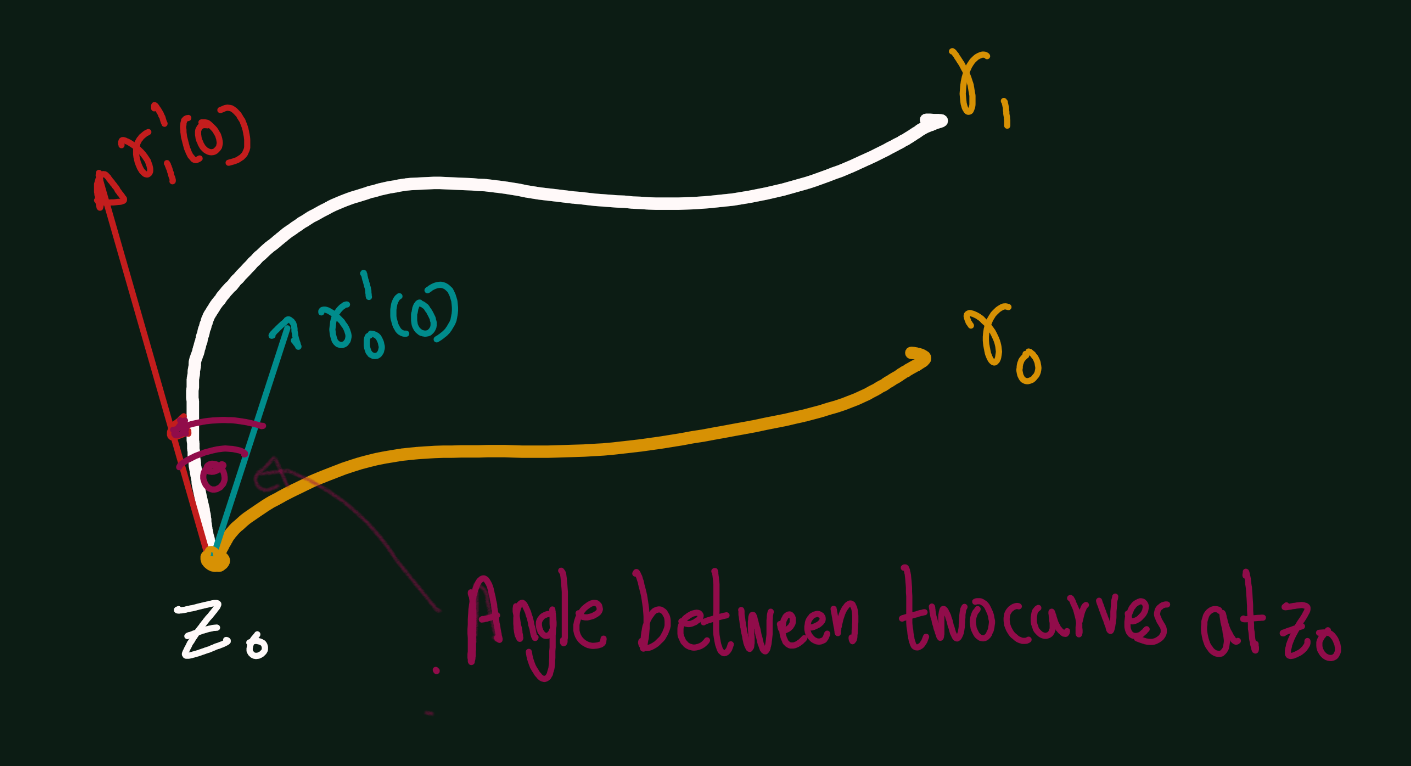
\includegraphics[width=19.6in]{figures/Confromal_mapping/fig1}

\begin{theorem}
\protect\hypertarget{thm:unnamed-chunk-22}{}\label{thm:unnamed-chunk-22}If \(\gamma(t)\), \(0 \leq t \leq 1\), is a smooth parameterized curve terminating at \(z_0 = \gamma(0)\), and \(f(z)\) is analytic at \(z_0\), then the tangent to the curve \(f(\gamma(t))\) terminating at \(f(z_0)\) is given by:
\begin{equation}
(f \circ \gamma)'(0) = f'(z_0)\gamma'(0)
\end{equation}
\end{theorem}

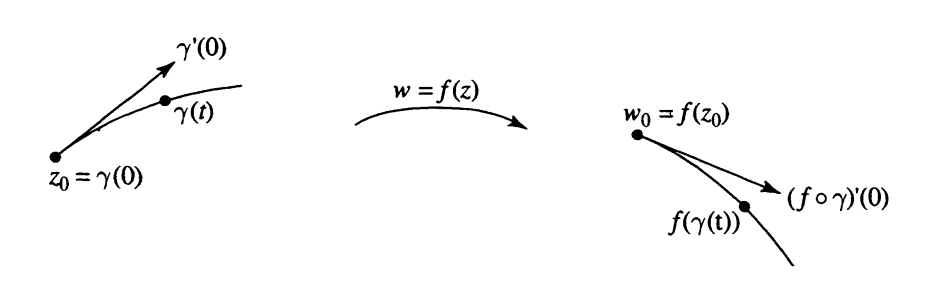
\includegraphics[width=13in]{figures/Confromal_mapping/fig2}

\begin{proof}
\leavevmode

\begin{itemize}
\tightlist
\item
  If \(\gamma'(0) \neq 0\), then \(\gamma(t) \neq \gamma(0)\) for \(t\) near \(0\), \(t \neq 0\), so we may write
  \begin{equation}
  \frac{f(\gamma(t)) - f(\gamma(0))}{t} = \frac{f(\gamma(t)) - f(\gamma(0))}{\gamma(t) - \gamma(0)} \cdot \frac{\gamma(t) - \gamma(0)}{t}
  \end{equation}
  and pass to the limit, to obtain the formula (6.1).
\item
  If \(\gamma'(0) = 0\), then proceeding as in Section 2, we obtain \((f \circ \gamma)'(0) = 0\), and again the formula holds.
\end{itemize}

\end{proof}

\chapter{Uniformization by square domains}\label{uniformization-by-square-domains}

\begin{definition}[Domain]
\protect\hypertarget{def:unnamed-chunk-25}{}\label{def:unnamed-chunk-25}A subset \(D\) of the complex plane is a domain if \(D\) is open and if any two points of \(D\) can be connected by a broken line segment in \(D\).
\end{definition}

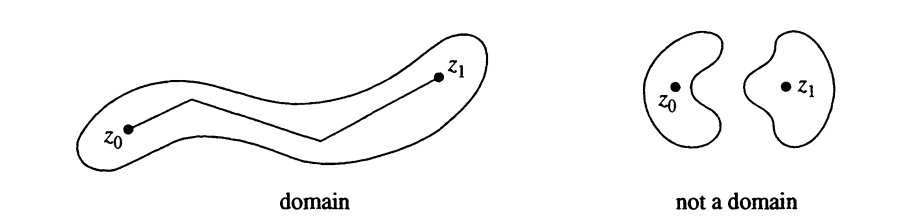
\includegraphics[width=12.58in]{figures/Mario_Bonk/fig1}

\begin{example}
\protect\hypertarget{exm:unnamed-chunk-27}{}\label{exm:unnamed-chunk-27}\leavevmode

\begin{itemize}
\tightlist
\item
  \textbf{Examples}:

  \begin{itemize}
  \tightlist
  \item
    Open half planes
  \item
    Open disks
  \item
    Open sectors
  \item
    Open annuli,
  \item
    Open punctured disks.
  \end{itemize}
\item
  \textbf{Non Examples}:

  \begin{itemize}
  \tightlist
  \item
    Union of the open upper and lower half-planes \(=U = \mathbb{C}\setminus\mathbb{R}\).\\
    (It is impossible to connect a point in the upper half-plane to a point in the lower half-plane by a broken line segment that does not cross the real line. )
  \end{itemize}
\end{itemize}

\end{example}

\begin{definition}[Riemann Sphere]
\protect\hypertarget{def:unnamed-chunk-28}{}\label{def:unnamed-chunk-28}The Riemann sphere, also called the extended complex plane consist of the complex numbers \(\mathbb{C}\) together with \(\infty\). The set of extended complex numbers may be written as \(\mathbb{C} \cup \{\infty\}\).
\end{definition}

\textbf{Notation}: \(\hat{\mathbb{C}}=\mathbb{C} \cup \{\infty\}\)

\begin{center}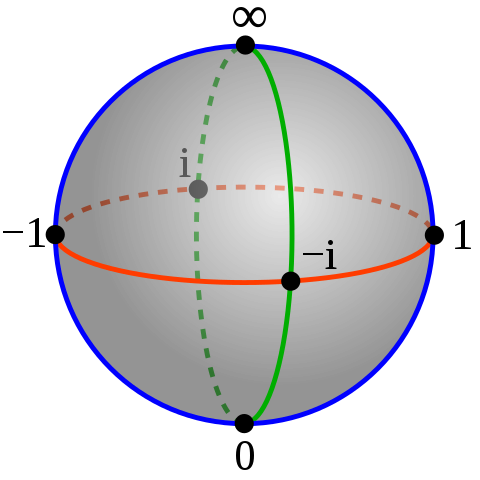
\includegraphics[width=6.67in,height=0.5\textheight]{figures/Mario_Bonk/fig2} \end{center}

\begin{definition}
\protect\hypertarget{def:unnamed-chunk-30}{}\label{def:unnamed-chunk-30}A domain in the plane is ``simply connected'' if it has no ``holes.''
\end{definition}

\begin{example}
\protect\hypertarget{exm:unnamed-chunk-31}{}\label{exm:unnamed-chunk-31}\leavevmode

\begin{itemize}
\tightlist
\item
  \textbf{Example}

  \begin{itemize}
  \tightlist
  \item
    Disks
  \item
    Rectangles
  \end{itemize}
\item
  *\textbf{Non Example}

  \begin{itemize}
  \tightlist
  \item
    Annuli
  \item
    Punctured disks
  \item
    Punctured plane\\
    (Becasue they have ``holes'')
  \end{itemize}
\end{itemize}

\end{example}

Later we discuss this more precise

\begin{definition}[Meromophic]
\protect\hypertarget{def:unnamed-chunk-32}{}\label{def:unnamed-chunk-32}A function \(f(z)\) is meromorphic on a domain \(D\) if \(f(z)\) is analytic on \(D\) except possibly at isolated singularities, each of which is a pole.
\end{definition}

\begin{proof}
(Proof of Therom 1.1 in th paper)\\
Let \(\Omega\) be a finitely connected domain in \(\hat{\mathbb{C}}\) with \(\infty\in \Omega\) It is a known fact that there exists a conformal map \(g\) of \(\Omega\) onto a square domain \(\tilde{\Omega}\) with the normalization
\[g(z) = z + \frac{b_1}{z} + \ldots\]
near \(\infty\).

The map \(f \in \mathcal{F} \mapsto \tilde{f} := f \circ g^{-1}\) is a bijection between \(\mathcal{F}\) and \(\tilde{\mathcal{F}}\). Moreover, if
\[f(z) = z + \frac{a_1}{z} + \ldots ~\text{ and } \tilde{f}(z) = z + \frac{\tilde{a_1}}{z} + \ldots\] near \(\infty\), then \(\tilde{a}_1 = a_1 - b_1\).
\end{proof}

Let \(f\) be as in the statement. We consider the rectangle \(R = [-l,l] \times [-r,r] \subset \mathbb{C}\) for large \(r > 0\). Here we chose \(l= = r^{2/3}\) so that
\[ \frac{l}{r} \to  0 \quad \text{and} \quad \frac{r}{l^2} \to 0\]
as \(r \to \infty\).

In the following, we assume that \(r\) is so large that \(\widetilde{C}\setminus \Omega\) is contained in the interior of \(R\). Then \(\partial R \subset \widetilde{C}\setminus \Omega\) and \(j=f(R)\) is a Jordan curve in \(\mathbb{C}\). We want to

\begin{eqnarray}
A &=& \frac{1}{2i} \int_J \bar{w} dw\\
&=& \frac{1}{2i} \int_{\partial R} \bar{f(z)}f'(z) dz\\
&=& \frac{1}{2i} \int_{\partial R} \overline{\left(z + \frac{a_1}{z} + \ldots \right)} \left(1 - \frac{a_1}{z^2} + \ldots \right) dz\\
&=& \frac{1}{2i} \int_{\partial R} \left(\bar{z} + \frac{\bar{a}_1}{\overline{z}}-\frac{\bar{a}_1\bar{z}}{z^2} + O\left(\frac{1}{|z|^2}\right)\right) dz\\
&=& 4rl + \int_{\partial R} \text{Im} \left(\frac{\bar{a}_1 z}{\bar{z}}\right) \frac{dz}{z} + o(1).
\end{eqnarray}

Sure, I can provide a proof for the proposition. Here it goes:

\textbf{Proposition}: If a set \(A\) is a subset of the interior of another set \(B\) (denoted as \(A \subseteq Int(B)\)), then the complement of \(A\) (denoted as \(A^c\)) is a subset of the boundary of \(B\) (denoted as \(bd(B)\)).

\textbf{Proof}:

Let's denote the interior of \(B\) as \(Int(B)\) and the boundary of \(B\) as \(bd(B)\). By definition, we have:

\begin{enumerate}
\def\labelenumi{\arabic{enumi}.}
\tightlist
\item
  \(Int(B) = B - bd(B)\)
\item
  \(A^c = U - A\) where \(U\) is the universal set.
\end{enumerate}

Given that \(A \subseteq Int(B)\), we can say that \(A\) does not contain any points from \(bd(B)\). Therefore, all points in \(bd(B)\) must be in \(A^c\).

Hence, \(A^c \subseteq bd(B)\).

This completes the proof. Please note that this is a general proof and the specifics might vary depending on the exact definitions and properties of the sets and the topological space they are in. If you have a specific example or further questions, feel free to ask!

\chapter{Riemann Mapping Theorem}\label{riemann-mapping-theorem}

\begin{theorem}[Riemann Mapping Theorem]
\protect\hypertarget{thm:unnamed-chunk-34}{}\label{thm:unnamed-chunk-34}If \(D\) is a simply connected domain in the complex plane, and \(D\) is not the entire complex plane, then there is a conformal map of \(D\) onto the open unit disk \(\mathbb{D}\).
\end{theorem}

\section{Hyperbolic Geomeery}\label{hyperbolic-geomeery}

Suppose \(w = f(z)\) is a conformal self-map of the open unit disk \(\mathbb{D}\). From Pick's lemma we then have equality,
\[\left|\frac{d\omega}{dz}\right|=\frac{1-|\omega|^2}{1-|z|^2}\]
In differential form this becomes
\[\frac{|dw|}{1-|w|^2} = \frac{|dz|}{1-|z|^2},\]
which means that if \(\gamma\) is any smooth curve in \(\mathbb{D}\), and \(\omega=f(z)\) is a conformal self-map of \(\mathbb{D}\), then
\[\int_{f\circ \gamma}\frac{|dw|}{1-|w|^2} =\int_{\gamma} \frac{|dz|}{1-|z|^2}.\]
Thus to obtain a length function that is invariant under conformal self-maps of \(\mathbb{D}\),we are led to make the following definition.

\begin{definition}
\protect\hypertarget{def:unnamed-chunk-35}{}\label{def:unnamed-chunk-35}We define the length of \(\gamma\) in the hyperbolic metric by
\[\text{hyperbolic length of } \gamma =2\int_{\gamma} \frac{|dz|}{1-|z|^2}\]
\end{definition}

The factor 2 is a harmless factor, which is often omitted. (It adjusts the
metric so that its curvature is -1.)

\begin{definition}
\protect\hypertarget{def:unnamed-chunk-36}{}\label{def:unnamed-chunk-36}The hyperbolic distance \(\rho(z_0, z_1)\) from \(z_0\) to \(z_1\) is defined as the infimum (greatest lower bound) of the hyperbolic lengths of all piecewise smooth curves in \(\mathbb{D}\) from \(z_0\) to \(z_1\).
\[\rho(z_0, z_1)
  =\inf_\gamma\left\{\text{hyperbolic length of } \gamma \right\}
  =\inf_\gamma\left\{2\int_{\gamma} \frac{|dz|}{1-|z|^2}\right\}\]
\end{definition}

\begin{center}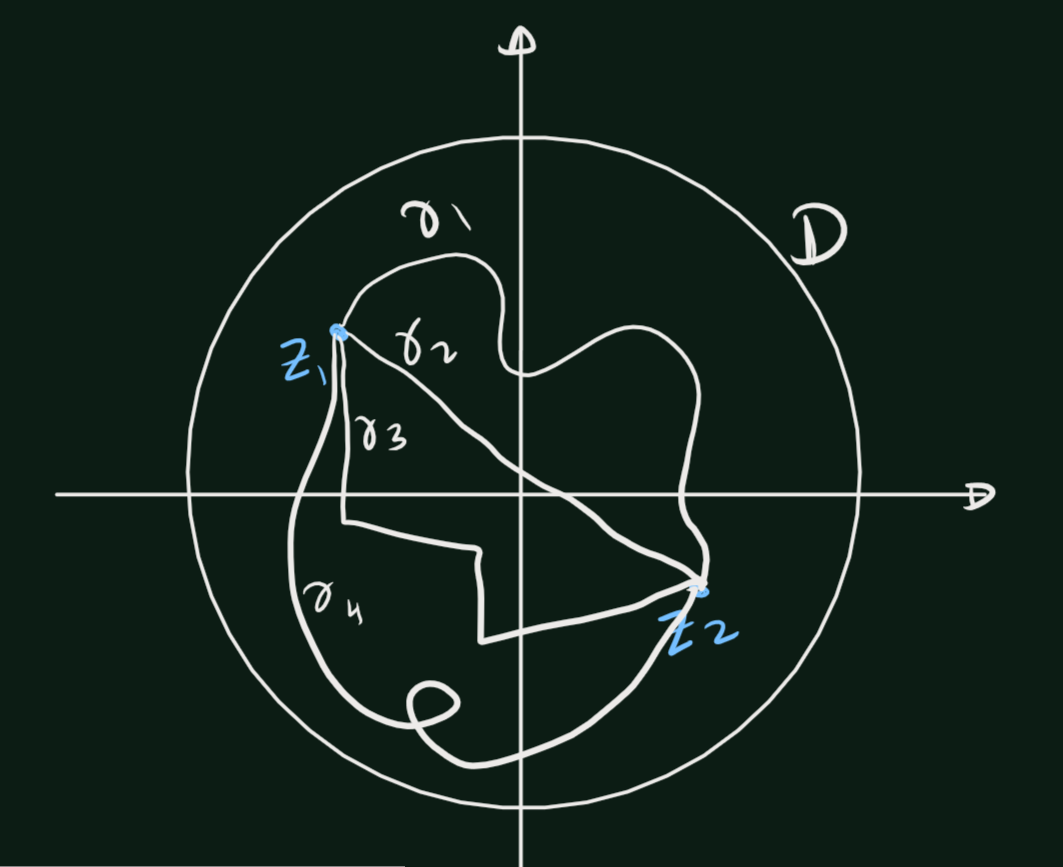
\includegraphics[width=14.76in]{figures/Riemann_Mapping_Therom/fig1} \end{center}

Since conformal self-maps of \(\mathbb{D}\) preserve the hyperbolic lengths of curves, they also preserve hyperbolic distances. That is, for any conformal self-map \(w = J(z)\) of \(\mathbb{D}\),
\[ \rho(f(z_0), f(z_1)) = \rho(z_0, z_1), \quad \text{where } z_0, z_1 \in \mathbb{D}. \]

\begin{center}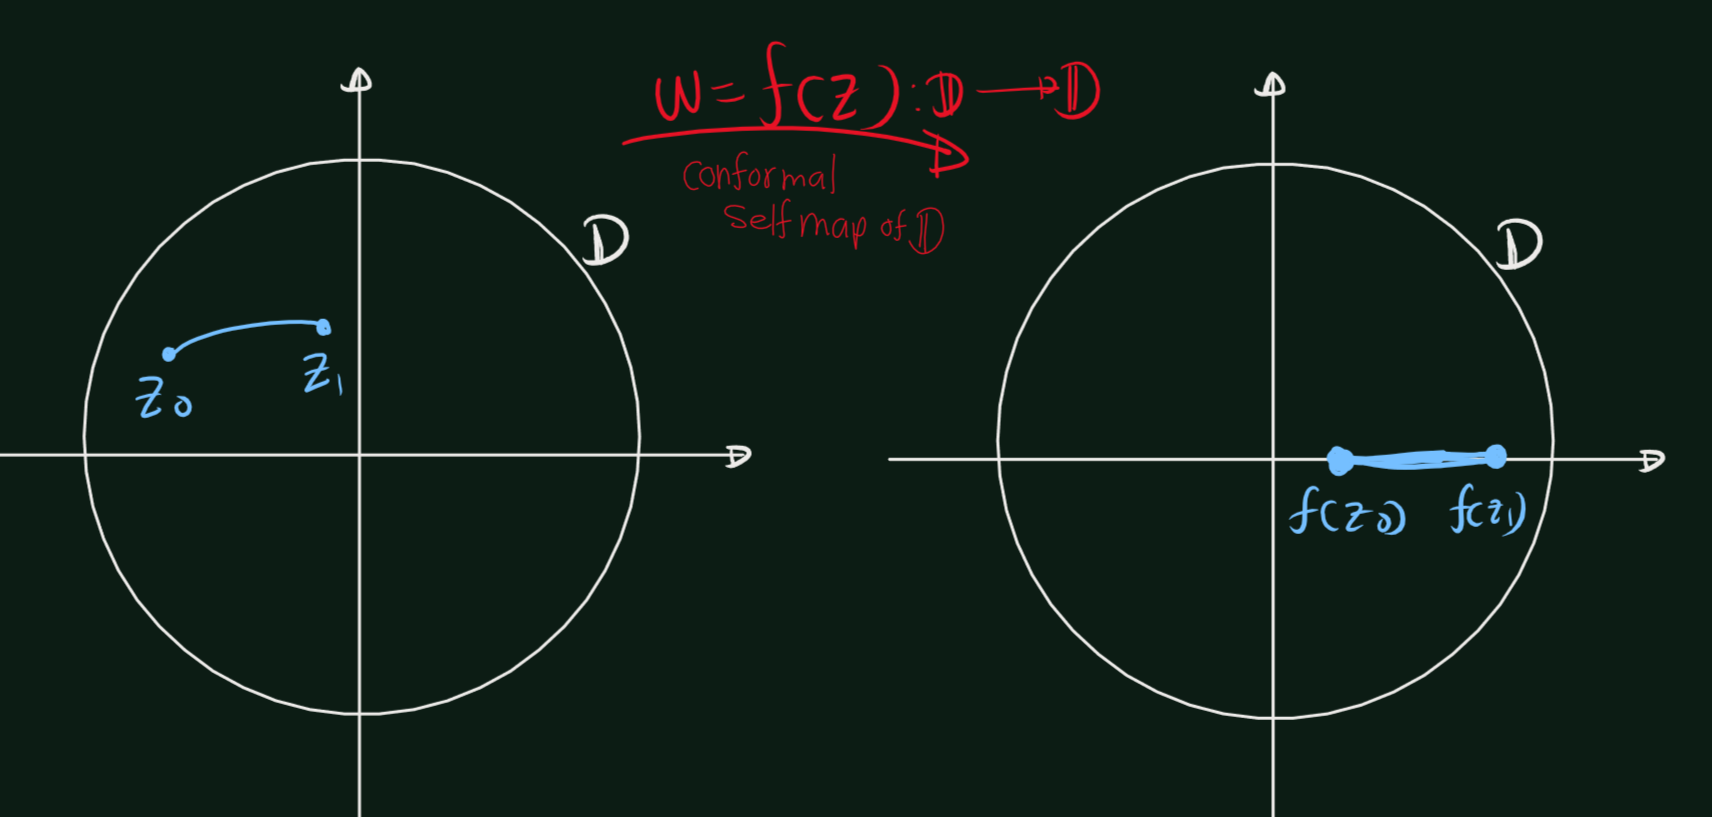
\includegraphics[width=23.78in]{figures/Riemann_Mapping_Therom/fig2} \end{center}

\begin{theorem}
\protect\hypertarget{thm:unnamed-chunk-39}{}\label{thm:unnamed-chunk-39}For any two distinct points \(z_0, z_1\) in the open unit disk \(\mathbb{D}\), there exists a unique shortest curve in \(\mathbb{D}\) from \(z_0\) to \(z_1\) in the hyperbolic metric. Specifically, this curve corresponds to the arc of the circle passing through \(z_0\) and \(z_1\) that is orthogonal to the unit circle.
\end{theorem}

\begin{definition}
\protect\hypertarget{def:unnamed-chunk-40}{}\label{def:unnamed-chunk-40}The paths of shortest hyperbolic length between points are called \textbf{hyperbolic geodesics}.
\end{definition}

\begin{itemize}
\tightlist
\item
  These hyperbolic geodesics play a role similar to that of straight lines in Euclidean geometry. They satisfy all the axioms of Euclidean geometry except for the parallel axiom (which states that through each point not on a given line, there passes a unique straight line through the point and parallel to the given line).
\end{itemize}

\begin{center}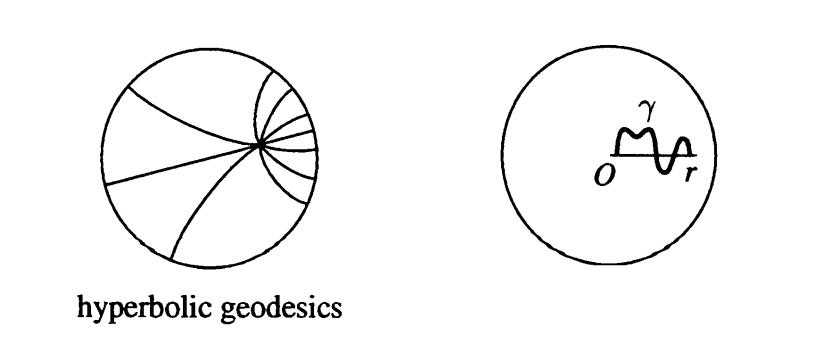
\includegraphics[width=11.5in]{figures/Riemann_Mapping_Therom/fig3} \end{center}

\begin{proof}
(proof of theorem), Let \(w = f(z)\) be a conformal self-map of \(\mathcal{D}\)
such that \(f(z_o) = 0\).
By multiplying by a unimodular constant, we can arrange that \(f(z_l) = r > 0\). Since \(f(z)\) preserves hyperbolic lengths, and since \(fx(z)\) maps circles orthogonal to the unit circle onto circles orthogonal to the unit circle, it suffices to show that the straight line segment from 0 to \(r\) is a unique path of shortest hyperbolic length from 0 to \(r\).
For this, let \(\gamma(t) = x(t) + iy(t)\), \(0 \leq t \leq 1\), be a piecewise smooth path in \(\mathbb{C}\) from 0 to \(r\).
Then \(alpha(t) = \Re(\gamma(t)) = x(t)\) defines a path in \(\mathbb{D}\) from 0 to \(r\) along the real axis, and
\[\int_\alpha \frac{|dz|}{1-|z|^2}=\int_0^1\frac{|dx(t)|}{1-(x(t))^2}\leq \int_0^1\frac{|dx(t)|}{1-(\gamma(t))^2}\leq \int_\gamma \frac{|dz|}{1-|z|^2}\]

If \(y(t) \neq 0\) for some \(t\), then \(|\gamma(t)| > |x(t)|\), and the first inequality above is strict. In this case, the path \(a(t)\) on the real axis is strictly shorter than the path \(\gamma(t)\). Further, if \(a(t)\) is decreasing on some interval, we could reduce the integral by deleting a parameter interval over which \(a(t)\) starts and ends at the same value. We conclude that the integral is a minimum exactly when \(\gamma(t)\) is real and nondecreasing, in which case the path is the straight line segment from 0 to \(r\).
\end{proof}

\begin{center}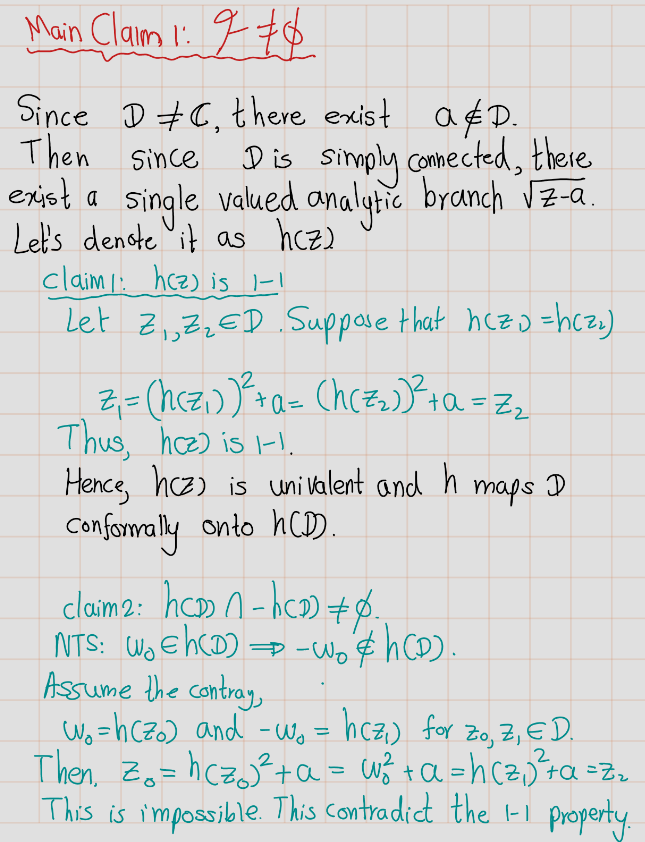
\includegraphics[width=8.96in]{figures/Riemann_Mapping_Therom/fig5} \end{center}

\section{Proof of Riemann Mapping Theorem}\label{proof-of-riemann-mapping-theorem}

Recall the following theorem.

\begin{theorem}
\protect\hypertarget{thm:thm1}{}\label{thm:thm1}

The following properties are equivalent, for a domain \(D\) in the complex plane:

\begin{enumerate}
\def\labelenumi{\roman{enumi}.}
\tightlist
\item
  \(D\) is simply connected,
\item
  every closed differential on \(D\) is exact,
\item
  for each \(z_0 \in \mathbb{C} \setminus D\), there is an analytic branch of \(\log(z - z_0)\) defined
  on \(D\),
\item
  each closed curve \(\gamma\) in \(D\) has winding number \(W(\gamma, z_0) = 0\) about all points \(z_0 \in \mathbb{C} \setminus D\),
\end{enumerate}

\begin{enumerate}
\def\labelenumi{(\alph{enumi})}
\setcounter{enumi}{21}
\tightlist
\item
  the complement of \(D\) in the extended complex plane \(\hat{\mathbb{C}}\) is connected.
\end{enumerate}

\end{theorem}

Suppose that \(D\) is simply connected and that \(D \neq \mathbb{C}\). Choose \(a \in \mathbb{C} \setminus D\). By the characterization of simple connectivity,
By theorem \ref{thm:thm1}, there is an analytic branch \(g(z)\) of \(\log(z - a)\) in \(D\).
Then,
\[h(z) = e^{g(z)/2}=e^{\left(\frac{log(z-a)}{2}\right)}=(z-a)^{\frac{1}{2}}=\sqrt{z-a}\]
So, \(h(z) = e^{g(z)/2}\) is an analytic branch of \(\sqrt{z - a}\) in \(D\), and \((h(z))^2 = z - a \neq 0\) (Since \(a\not\in D\)) in \(D\). If \(h(z_1) = h(z_2)\), then \[z_1 = (h(z_1))^2 + a = (h(z_2))^2 + a = z_2\].
Thus \(h(z)\) is univalent, and \(h(z)\) maps \(D\) conformally onto \(h(D)\). Finally, note that if \(w_0 \in h(D)\), then \(-w_0 \notin h(D)\). Indeed, if \(w_0 = h(z_0)\) and \(-w_0 = h(z_1)\) for \(z_0, z_1 \in D\), then \(z_0 = h(z_0)^2 + a = w_0^2 + a = h(z_1)^2 + a = z_1\), which is impossible. We summarize.

\begin{lemma}
\protect\hypertarget{lem:unnamed-chunk-44}{}\label{lem:unnamed-chunk-44}Let \(D\) be a simply connected domain. Suppose \(a \notin D\), and let
\(h(z)\) be an analytic branch of \(\sqrt{z - a}\) in \(D\). Then \(h(z)\) is univalent on \(D\), and further, \(h(D)\) is disjoint from \(-h(D)\).
\end{lemma}

\begin{proof}
Done it earler.
\end{proof}

\subsection{Adlof Proof}\label{adlof-proof}

\begin{theorem}[Riemann Mapping Theorem]
\protect\hypertarget{thm:unnamed-chunk-46}{}\label{thm:unnamed-chunk-46}Given any simply connected region \(\Omega\) which is not the whole plane, and a point \(z_0\) in \(\Omega\), there exists a unique analytic function \(f(z)\) in \(\Omega\), normalized by the conditions \(f(z_0) = 0\), \(f'(z_0) > 0\), such that \(f(z)\) defines a one-to-one mapping of \(\Omega\) onto the unit disk \(\mathbb{D}=\{|w| < 1\}\).
\end{theorem}

\begin{center}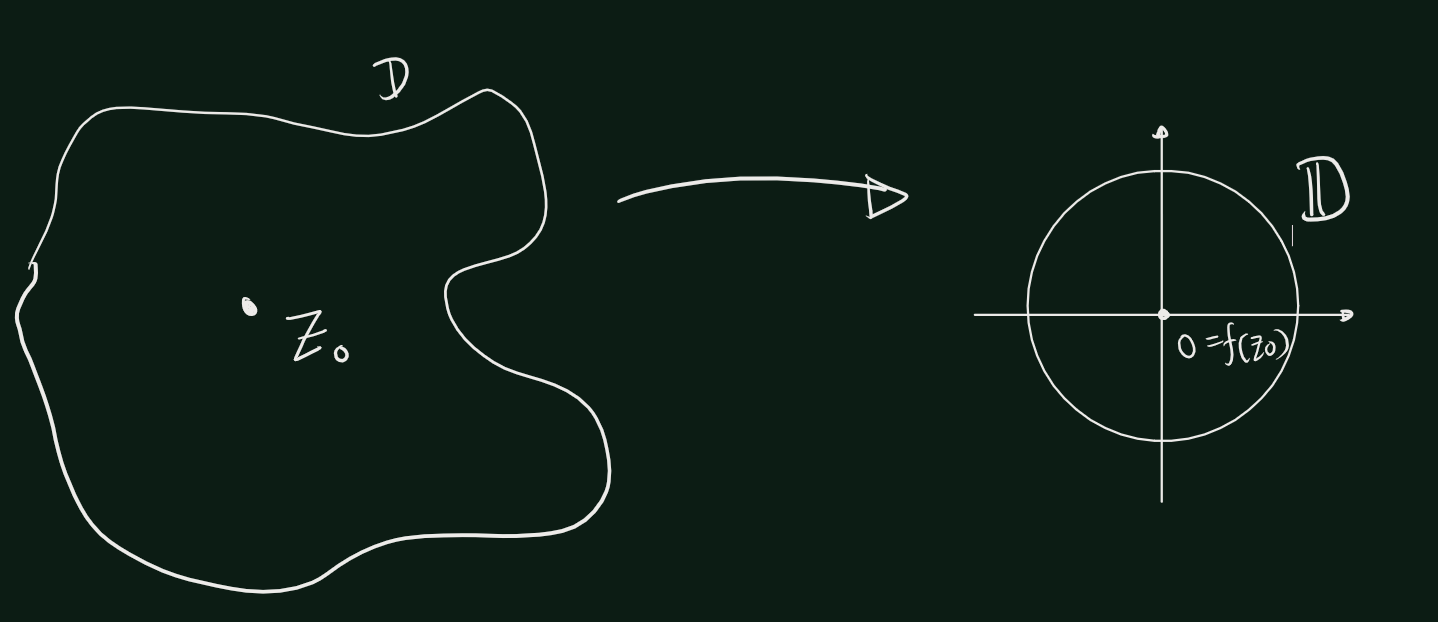
\includegraphics[width=19.97in]{figures/Riemann_Mapping_Therom/fig4} \end{center}

\emph{Proof.}
First fix \(z_0\). Let \(\mathcal{F}\) be the family of univalent functions on \(D\) such that \(|f(z)|\leq 1\) on \(D\) and \(f(z_0)=0\) for all \(f \in \mathcal{F}\). We proceed with the proof here in four parts

\begin{enumerate}
\def\labelenumi{\roman{enumi}.}
\tightlist
\item
  \(\mathcal{F}\) is non-empty.
\item
  \(|f'(z_0)|\) is bounded above for all \(f\in \mathcal{F}\).
\item
  There exist \(g\in \mathcal{F}\) such that \(|g'(z)|\) is maximal
\item
  The function \(g\) is a biholomorphic map from \(D\) to \(\mathbb{D}\)
\end{enumerate}

\begin{center}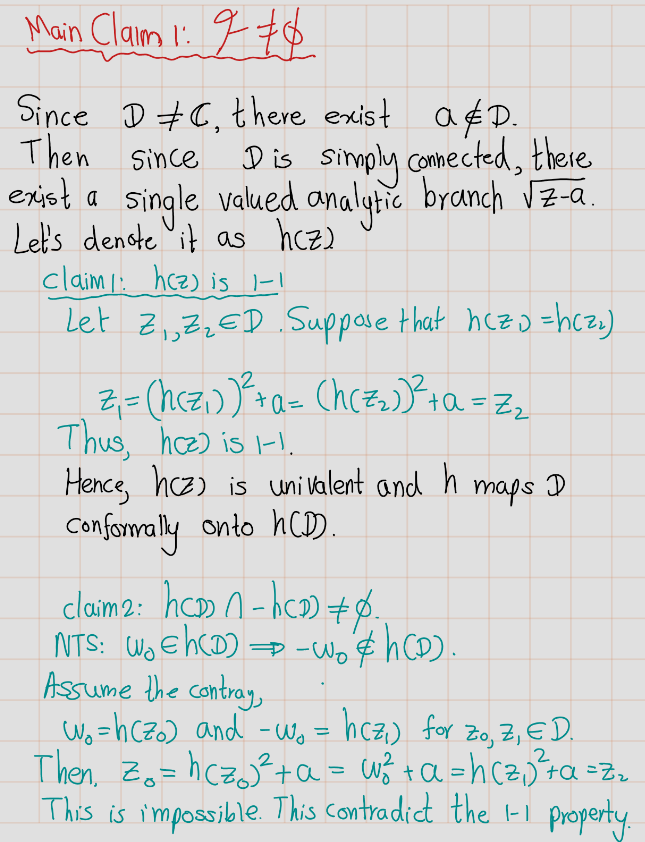
\includegraphics[width=8.96in]{figures/Riemann_Mapping_Therom/fig5} \end{center}

\begin{center}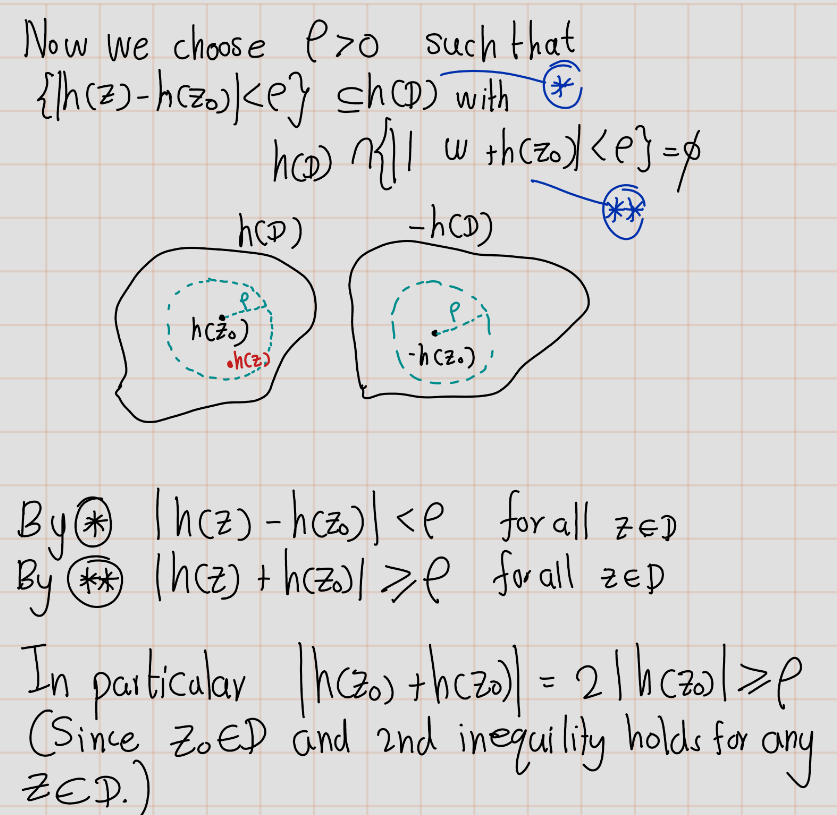
\includegraphics[width=11.62in]{figures/Riemann_Mapping_Therom/fig6} \end{center}

\begin{center}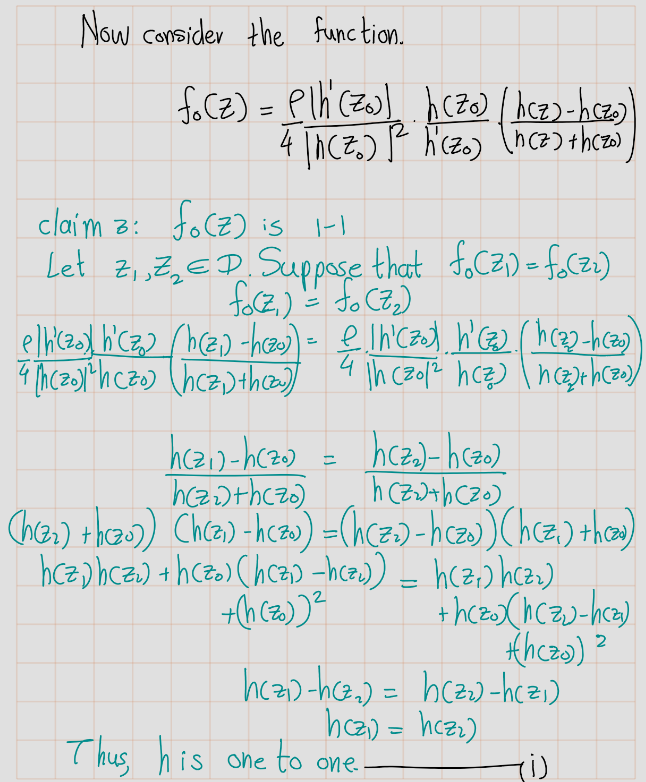
\includegraphics[width=8.97in]{figures/Riemann_Mapping_Therom/fig7} \end{center}

\begin{center}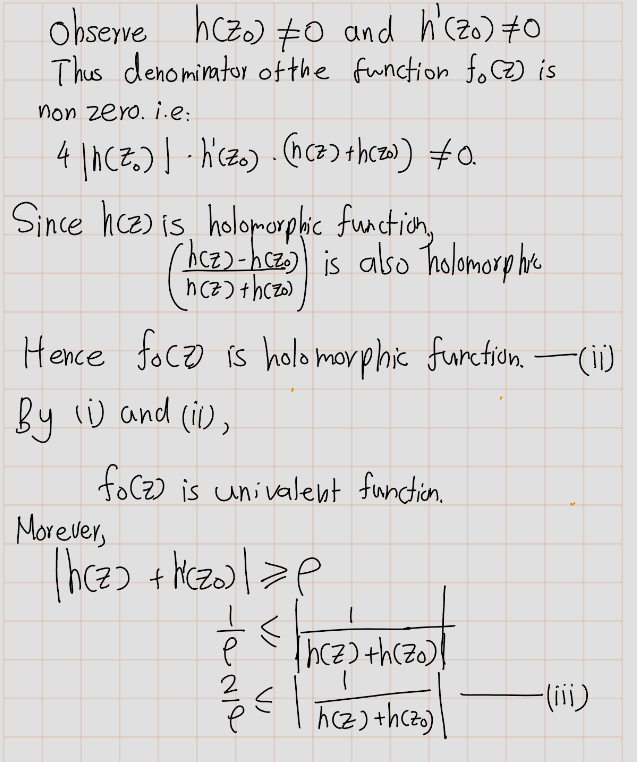
\includegraphics[width=8.85in]{figures/Riemann_Mapping_Therom/fig8} \end{center}

\begin{center}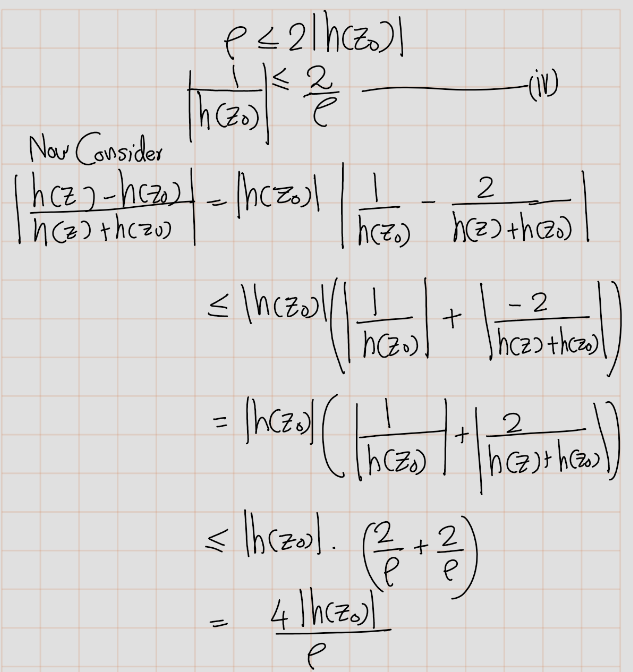
\includegraphics[width=8.79in]{figures/Riemann_Mapping_Therom/fig9} \end{center}

\begin{center}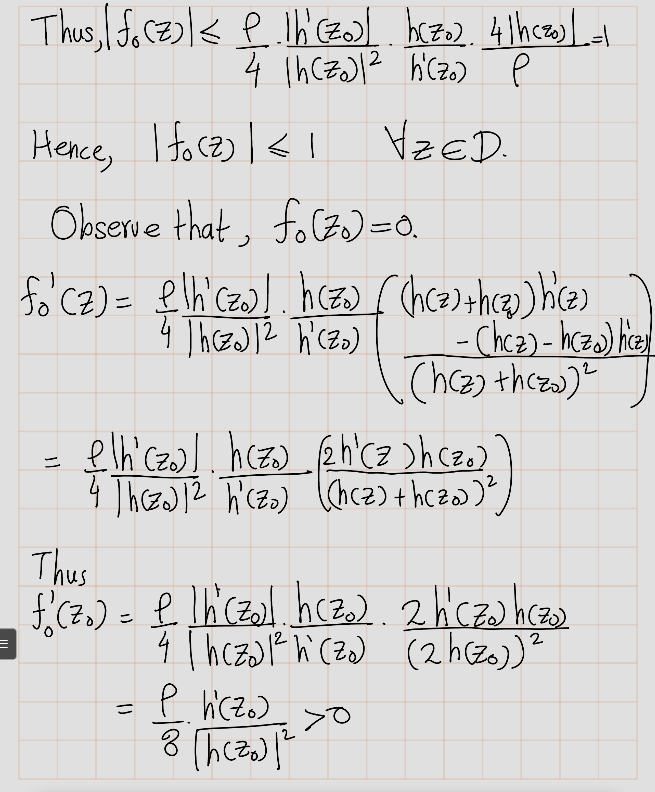
\includegraphics[width=9.1in]{figures/Riemann_Mapping_Therom/fig10} \end{center}

\begin{center}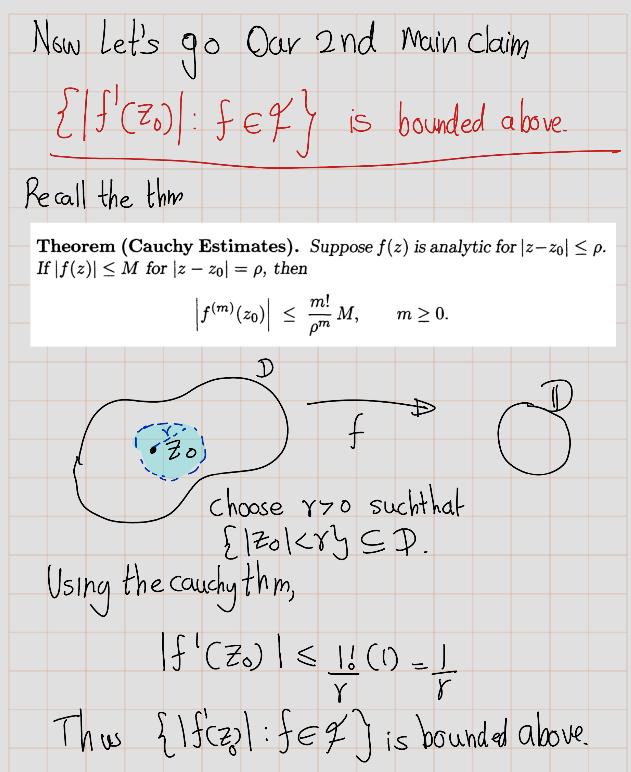
\includegraphics[width=8.76in]{figures/Riemann_Mapping_Therom/fig11} \end{center}

\begin{center}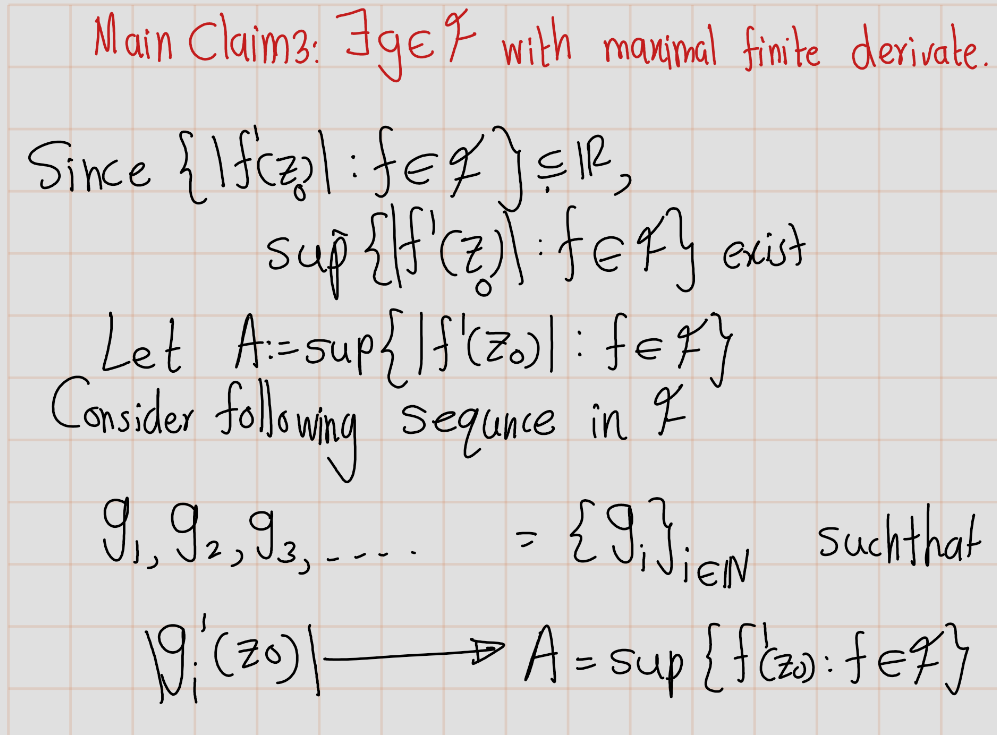
\includegraphics[width=13.85in]{figures/Riemann_Mapping_Therom/fig12} \end{center}

\begin{theorem}[Montel Theorem]
\protect\hypertarget{thm:unnamed-chunk-56}{}\label{thm:unnamed-chunk-56}Suppose \(F\) is a family of analytic functions on a domain \(D\) such that \(F\) is uniformly bounded on each compact subset of \(D\). Then every sequence in \(F\) has a subsequence that converges normally on \(D\), that is, uniformly on each compact subset of \(D\).
\end{theorem}

\begin{center}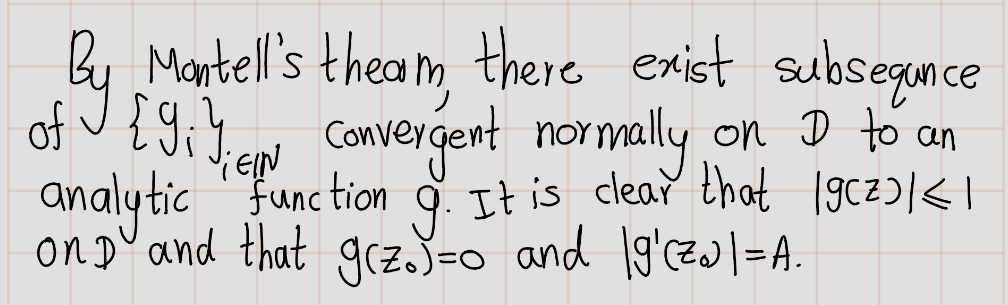
\includegraphics[width=14in]{figures/Riemann_Mapping_Therom/fig13} \end{center}

\section{LaTeX}\label{latex}

Given any simply connected region \(\Omega\) which is not the whole plane, and a point \(z_0\) in \(\Omega\), there exists a unique analytic function \(f(z)\) in \(\Omega\), normalized by the conditions \(f(z_0) = 0\), \(f'(z_0) > 0\), such that \(f(z)\) defines a one-to-one mapping of \(\Omega\) onto the disk \(|w| < 1\). The uniqueness is easily proved: if \(h\) and \(f_2\) are two such functions, then \(f_2 \circ h(w)\) defines a one-to-one mapping of \(|w| < 1\) onto itself. We know that such a mapping is given by a linear transformation \(S\) (Chapter 4, Section 3.4, Example 5). The conditions \(S(0) = 0\), \(S'(0) > 0\) imply \(S(w) = w\); hence, \(f = h \circ S\).

An analytic function \(g(z)\) in \(\Omega\) is said to be univalent if \(g(z_1) = g(z_2)\) only for \(z_1 = z_2\), in other words, if the mapping by \(g\) is one-to-one (the German word ``schlicht,'' which lacks an adequate translation, is also in common use). For the existence proof, we consider the family \(\mathcal{F}\) formed by all functions \(g\) with the following properties:
1. \(g\) is analytic and univalent in \(\Omega\).
2. \(|g(z)| \leq 1\) in \(\Omega\).
3. \(g(z_0) = 0\) and \(g'(z_0) > 0\).

We contend that \(f\) is the function in \(\mathcal{F}\) for which the derivative \(f'(z_0)\) is a maximum. The proof consists of three parts:
1. It is shown that the family \(\mathcal{F}\) is not empty.
2. There exists an \(f\) with maximal derivative.
3. This \(f\) has the desired properties.

To prove that \(\mathcal{F}\) is not empty, we note that there exists, by assumption, a point \(a \notin \Omega\). Since \(\Omega\) is simply connected, it is possible to define a single-valued branch of \(\sqrt{z - a}\) in \(\Omega\); denote it by \(h(z)\). This function does not take the same value twice, nor does it take opposite values. The image of \(\Omega\) under the mapping \(h\) covers a disk \(|w - h(z_0)| < p\), and therefore it does not meet the disk \(|w + h(z_0)| < p\). In other words, \(|h(z)| + |h(z_0)| \leq p\) for \(z \in \Omega\), and in particular, \(2|h(z_0)| \leq p\). It can now be verified that the function
\[ g_0(z) = \frac{1}{4|h(z_0)|^2} \left(h(z) - h(z_0)\right) \left(h'(z_0) h(z) + h(z_0)\right) \]
belongs to the family \(\mathcal{F}\). Indeed, because it is obtained from the univalent function \(h\) by means of a linear fractional transformation, it satisfies the desired properties.

\chapter{Codes}\label{codes}

\section{Python Code}\label{python-code}

\begin{Shaded}
\begin{Highlighting}[]
\ImportTok{import}\NormalTok{ matplotlib.pyplot }\ImportTok{as}\NormalTok{ plt}
\ImportTok{import}\NormalTok{ numpy }\ImportTok{as}\NormalTok{ np}

\KeywordTok{def}\NormalTok{ func(z):}
    \ControlFlowTok{return}\NormalTok{ z}\OperatorTok{**}\DecValTok{2}


\KeywordTok{def}\NormalTok{ plot\_conformal\_map(f, xmin, xmax, ymin, ymax, nb\_grid, nb\_points):}
\NormalTok{    xv, yv }\OperatorTok{=}\NormalTok{ np.meshgrid(np.linspace(xmin, xmax, nb\_grid), np.linspace(ymin, ymax, nb\_points))}
\NormalTok{    xv }\OperatorTok{=}\NormalTok{ np.transpose(xv)}
\NormalTok{    yv }\OperatorTok{=}\NormalTok{ np.transpose(yv)}

\NormalTok{    zv }\OperatorTok{=}\NormalTok{ func(xv }\OperatorTok{+} \OtherTok{1j}\OperatorTok{*}\NormalTok{yv)}
\NormalTok{    uv }\OperatorTok{=}\NormalTok{ np.real(zv)}
\NormalTok{    vv }\OperatorTok{=}\NormalTok{ np.imag(zv)}

\NormalTok{    xh, yh }\OperatorTok{=}\NormalTok{ np.meshgrid(np.linspace(xmin, xmax, nb\_points), np.linspace(ymin, ymax, nb\_grid))}

\NormalTok{    zh }\OperatorTok{=}\NormalTok{ func(xh }\OperatorTok{+} \OtherTok{1j}\OperatorTok{*}\NormalTok{yh)}
\NormalTok{    uh }\OperatorTok{=}\NormalTok{ np.real(zh)}
\NormalTok{    vh }\OperatorTok{=}\NormalTok{ np.imag(zh)}

\NormalTok{    ax }\OperatorTok{=}\NormalTok{ plt.subplot(}\DecValTok{121}\NormalTok{)}
    \ControlFlowTok{for}\NormalTok{ i }\KeywordTok{in} \BuiltInTok{range}\NormalTok{(}\BuiltInTok{len}\NormalTok{(yv)):}
\NormalTok{        ax.plot(xv[i], yv[i], }\StringTok{\textquotesingle{}b{-}\textquotesingle{}}\NormalTok{, lw}\OperatorTok{=}\DecValTok{1}\NormalTok{)}
\NormalTok{        ax.plot(xh[i], yh[i], }\StringTok{\textquotesingle{}r{-}\textquotesingle{}}\NormalTok{, lw}\OperatorTok{=}\DecValTok{1}\NormalTok{)}

\NormalTok{    ax2 }\OperatorTok{=}\NormalTok{ plt.subplot(}\DecValTok{122}\NormalTok{)}
    \ControlFlowTok{for}\NormalTok{ i }\KeywordTok{in} \BuiltInTok{range}\NormalTok{(}\BuiltInTok{len}\NormalTok{(vv)):}
\NormalTok{        ax2.plot(uv[i], vv[i], }\StringTok{\textquotesingle{}b{-}\textquotesingle{}}\NormalTok{, lw}\OperatorTok{=}\DecValTok{1}\NormalTok{)}
\NormalTok{        ax2.plot(uh[i], vh[i], }\StringTok{\textquotesingle{}r{-}\textquotesingle{}}\NormalTok{, lw}\OperatorTok{=}\DecValTok{1}\NormalTok{)}

\NormalTok{    plt.show()}


\NormalTok{nb\_grid }\OperatorTok{=} \DecValTok{9}
\NormalTok{nb\_points }\OperatorTok{=} \DecValTok{30}

\NormalTok{xmin, xmax, ymin, ymax }\OperatorTok{=} \OperatorTok{{-}}\DecValTok{1}\NormalTok{, }\DecValTok{1}\NormalTok{, }\OperatorTok{{-}}\DecValTok{1}\NormalTok{, }\DecValTok{1}

\NormalTok{plot\_conformal\_map(func, xmin, xmax, ymin, ymax, nb\_grid, nb\_points)}
\end{Highlighting}
\end{Shaded}

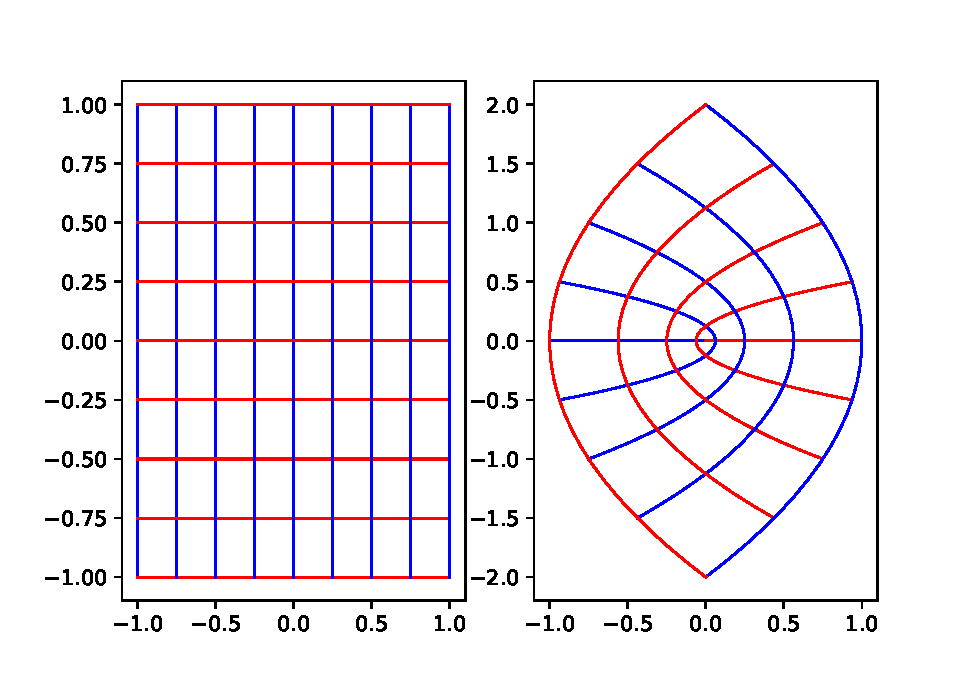
\includegraphics{ConformalMapping_files/figure-latex/unnamed-chunk-58-1.pdf}

\section{Helical Domain}\label{helical-domain}

\begin{Shaded}
\begin{Highlighting}[]
\CommentTok{\# The Logrithm Arc depend on the Constant theta and c}
\NormalTok{theta}\OtherTok{\textless{}{-}}\DecValTok{1}
\NormalTok{c}\OtherTok{\textless{}{-}}\DecValTok{2}


\NormalTok{x}\OtherTok{\textless{}{-}}\FunctionTok{seq}\NormalTok{(}\SpecialCharTok{{-}}\DecValTok{10}\NormalTok{,}\DecValTok{10}\NormalTok{,}\AttributeTok{length.out=}\DecValTok{1000}\NormalTok{)}
\NormalTok{y}\OtherTok{\textless{}{-}}\FunctionTok{seq}\NormalTok{(}\SpecialCharTok{{-}}\DecValTok{10}\NormalTok{,}\DecValTok{10}\NormalTok{,}\AttributeTok{length.out=}\DecValTok{1000}\NormalTok{)}
\NormalTok{z}\OtherTok{\textless{}{-}}\FunctionTok{outer}\NormalTok{(x,y,}\ControlFlowTok{function}\NormalTok{(x,y) }\FunctionTok{log}\NormalTok{(x}\SpecialCharTok{\^{}}\DecValTok{2} \SpecialCharTok{+}\NormalTok{ y}\SpecialCharTok{\^{}}\DecValTok{2}\NormalTok{)}\SpecialCharTok{*}\FunctionTok{sin}\NormalTok{(theta) }\SpecialCharTok{+} \FunctionTok{atan}\NormalTok{(y}\SpecialCharTok{/}\NormalTok{x)}\SpecialCharTok{*}\FunctionTok{cos}\NormalTok{(theta) }\SpecialCharTok{{-}}\NormalTok{c)}
\FunctionTok{contour}\NormalTok{(x,y,z,}\AttributeTok{nlevels=}\DecValTok{0}\NormalTok{)}
\end{Highlighting}
\end{Shaded}

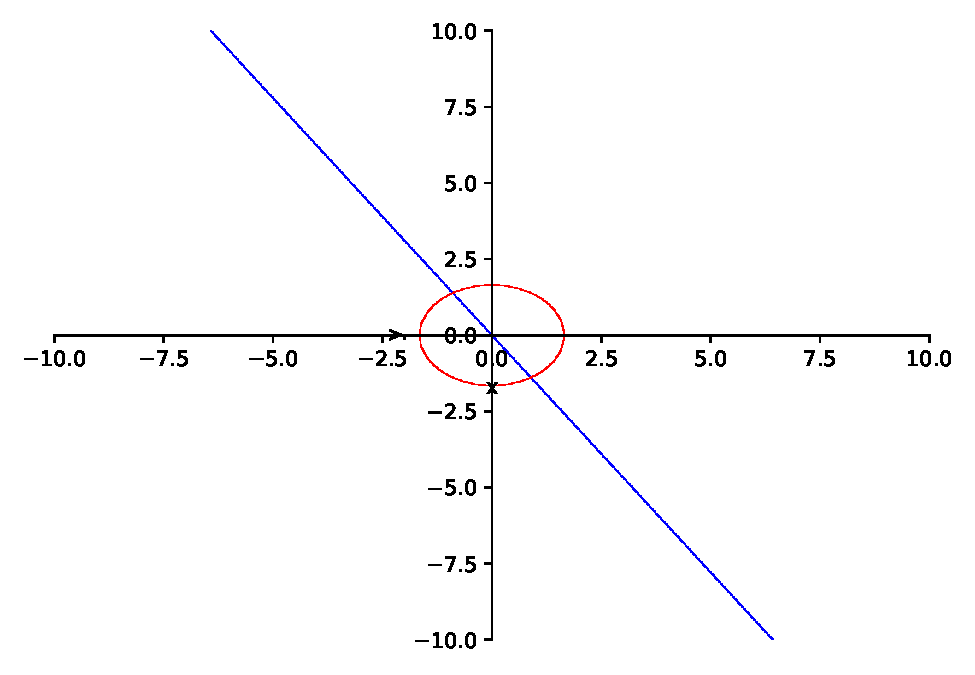
\includegraphics{ConformalMapping_files/figure-latex/unnamed-chunk-59-3.pdf}

\begin{Shaded}
\begin{Highlighting}[]
\ImportTok{from}\NormalTok{ sympy }\ImportTok{import} \OperatorTok{*}
\NormalTok{theta}\OperatorTok{=}\DecValTok{1}
\NormalTok{c}\OperatorTok{=}\DecValTok{2}
\NormalTok{x, y }\OperatorTok{=}\NormalTok{ symbols(}\StringTok{\textquotesingle{}x y\textquotesingle{}}\NormalTok{)}
\CommentTok{\#plot\_implicit(x**3 + x**2 {-} y**2, (x, {-}2, 2), (y, {-}2, 2))}
\NormalTok{plot\_implicit(log(x}\OperatorTok{**}\DecValTok{2} \OperatorTok{+}\NormalTok{ y}\OperatorTok{**}\DecValTok{2}\NormalTok{)}\OperatorTok{*}\NormalTok{sin(theta) }\OperatorTok{+}\NormalTok{ atan(y}\OperatorTok{/}\NormalTok{x)}\OperatorTok{*}\NormalTok{cos(theta) }\OperatorTok{{-}}\NormalTok{c,}
\NormalTok{(x, }\OperatorTok{{-}}\DecValTok{10}\NormalTok{, }\DecValTok{10}\NormalTok{), (y, }\OperatorTok{{-}}\DecValTok{10}\NormalTok{, }\DecValTok{10}\NormalTok{))}
\end{Highlighting}
\end{Shaded}

\begin{verbatim}
## <sympy.plotting.plot.Plot object at 0x000001D77F5D7B20>
\end{verbatim}

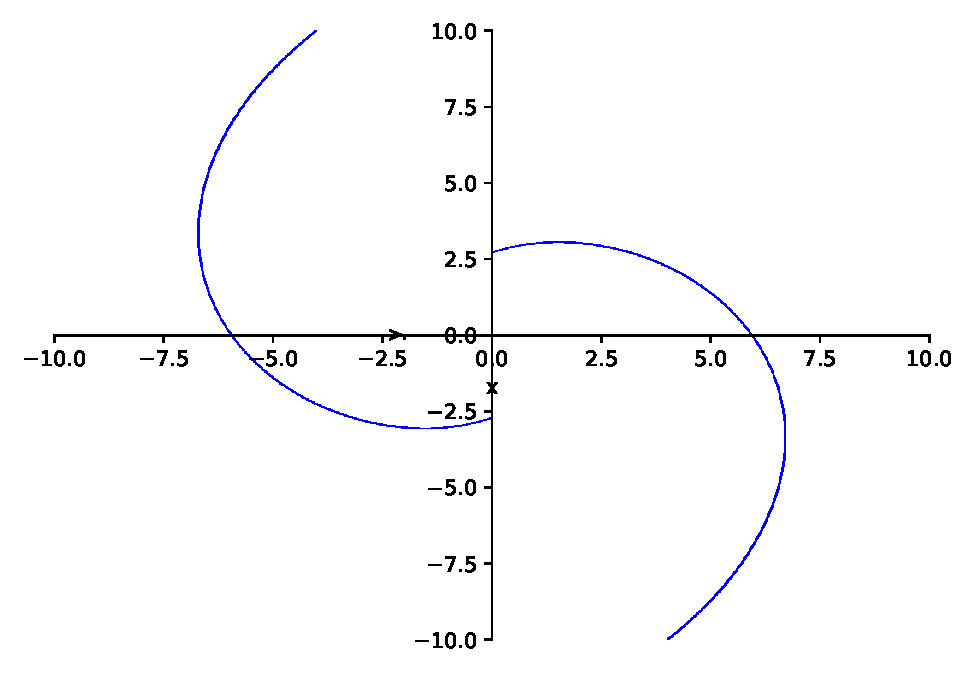
\includegraphics{ConformalMapping_files/figure-latex/unnamed-chunk-60-1.pdf}

\chapter{Helical Domain}\label{helical-domain-1}

In an analogous manner, we shall find the answer to the question of univalent mapping of multiply connected domains onto a plane with cuts along arcs of logarithmic spirals and, as limiting cases, onto the plane with radial cuts and with cuts along circular arcs of concentric circles.

For constant \(\theta\) and \(c\), the equation \(\Im(e^{-i\theta}\log(\xi))=c\) defines a logarithmic spiral in the \(\xi\)-plane with asymptotic point at the origin.This spiral has the property that it is intersected by an arbitrary ray issuing from the origin at an angle \(\theta\). This follows, for example, from the fact that if we shift to the plane \(t = \log(\xi)\), this logarithmic spiral is mapped into the straight line \(e^{-i\theta t} = c\) with inclination \(\theta\) to the real axis, and the ray referred to is mapped into a straight line parallel to the real axis.

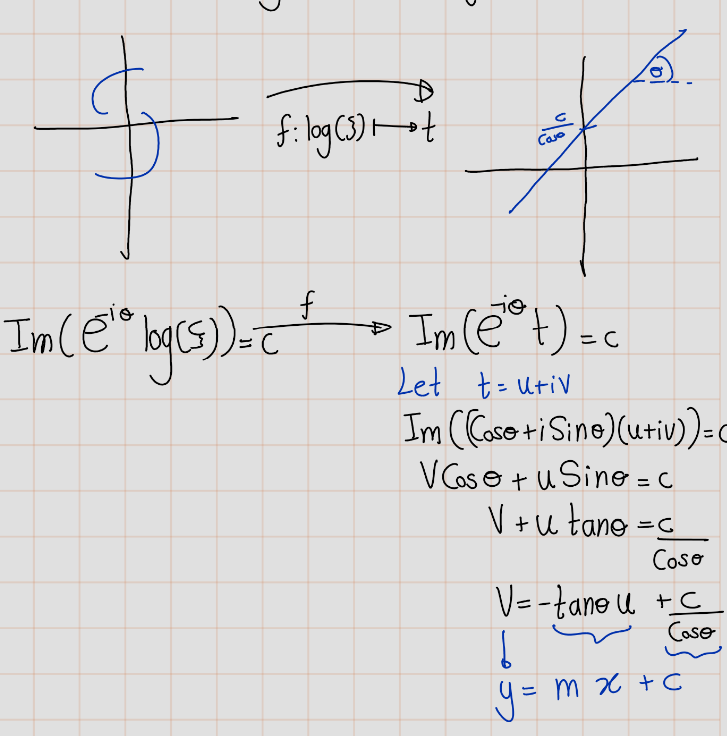
\includegraphics[width=10.1in]{figures/Helical_Domain/fig1}

\begin{itemize}
\tightlist
\item
  For \(\theta = 0\), the logarithmic spiral degenerates into a ray issuing from the origin.
\end{itemize}

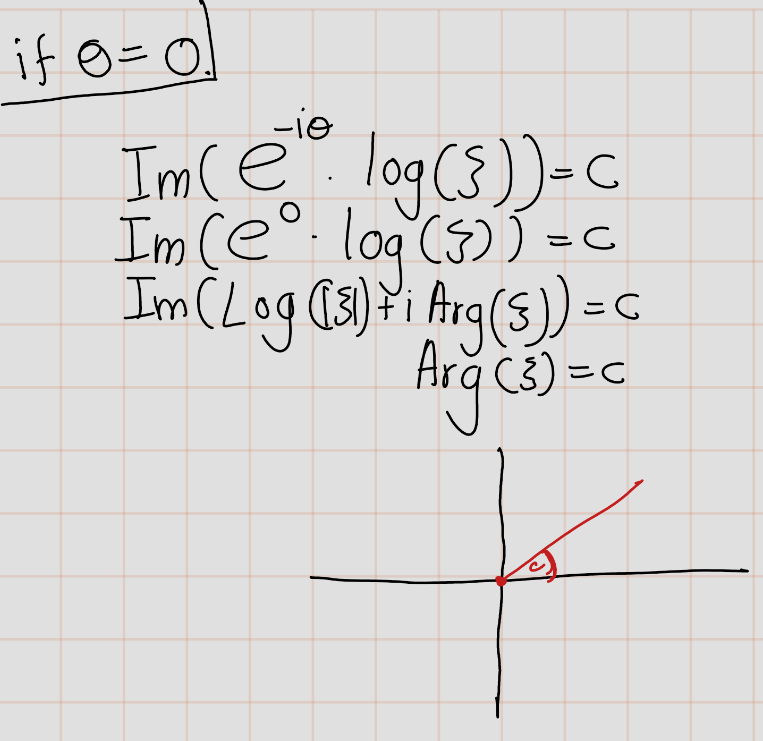
\includegraphics[width=10.6in]{figures/Helical_Domain/fig2}

\begin{Shaded}
\begin{Highlighting}[]
\ImportTok{from}\NormalTok{ sympy }\ImportTok{import} \OperatorTok{*}

\CommentTok{\# The Logrithm Arc depend on the Constant theta and c}
\NormalTok{theta}\OperatorTok{=}\DecValTok{0}
\NormalTok{c}\OperatorTok{=}\DecValTok{1}

\NormalTok{x, y }\OperatorTok{=}\NormalTok{ symbols(}\StringTok{\textquotesingle{}x y\textquotesingle{}}\NormalTok{)}

\NormalTok{plot\_implicit(log(x}\OperatorTok{**}\DecValTok{2} \OperatorTok{+}\NormalTok{ y}\OperatorTok{**}\DecValTok{2}\NormalTok{)}\OperatorTok{*}\NormalTok{sin(theta) }\OperatorTok{+}\NormalTok{ atan(y}\OperatorTok{/}\NormalTok{x)}\OperatorTok{*}\NormalTok{cos(theta) }\OperatorTok{{-}}\NormalTok{c,}
\NormalTok{(x, }\OperatorTok{{-}}\DecValTok{10}\NormalTok{, }\DecValTok{10}\NormalTok{), (y, }\OperatorTok{{-}}\DecValTok{10}\NormalTok{, }\DecValTok{10}\NormalTok{))}
\end{Highlighting}
\end{Shaded}

\begin{verbatim}
## <sympy.plotting.plot.Plot object at 0x000001D77F6B2230>
\end{verbatim}

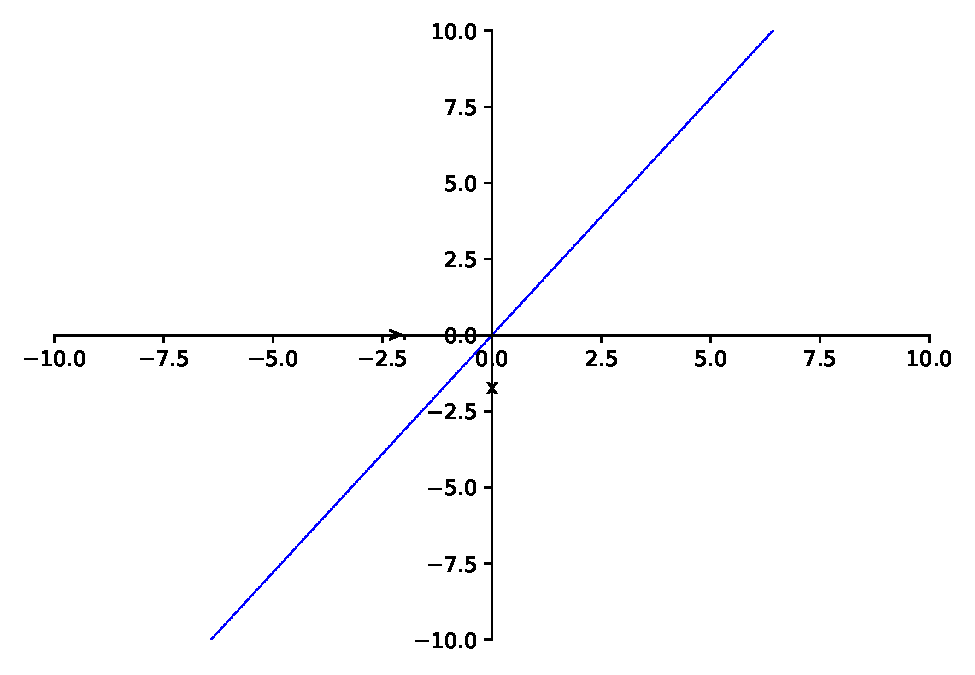
\includegraphics{ConformalMapping_files/figure-latex/unnamed-chunk-63-1.pdf}

\begin{itemize}
\tightlist
\item
  For \(\theta = \frac{\pi}{2}\), it degenerates to a circle with center at the origin.
\end{itemize}

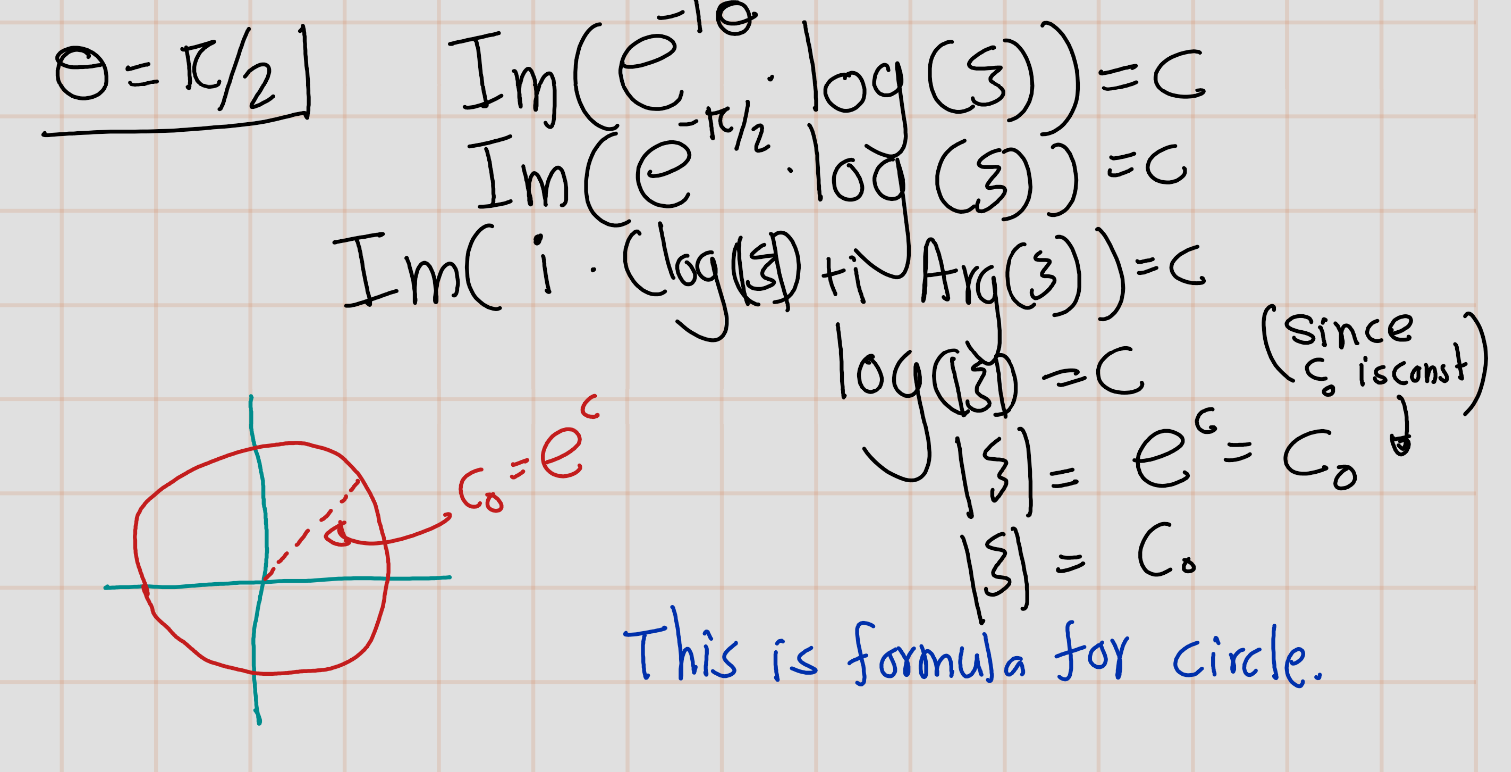
\includegraphics[width=20.99in]{figures/Helical_Domain/fig3}

\begin{Shaded}
\begin{Highlighting}[]
\ImportTok{from}\NormalTok{ sympy }\ImportTok{import} \OperatorTok{*}

\CommentTok{\# The Logrithm Arc depend on the Constant theta and c}
\NormalTok{theta}\OperatorTok{=}\NormalTok{pi}\OperatorTok{/}\DecValTok{2}
\NormalTok{c}\OperatorTok{=}\DecValTok{2}

\NormalTok{x, y }\OperatorTok{=}\NormalTok{ symbols(}\StringTok{\textquotesingle{}x y\textquotesingle{}}\NormalTok{)}

\NormalTok{plot\_implicit(log(x}\OperatorTok{**}\DecValTok{2} \OperatorTok{+}\NormalTok{ y}\OperatorTok{**}\DecValTok{2}\NormalTok{)}\OperatorTok{*}\NormalTok{sin(theta) }\OperatorTok{+}\NormalTok{ atan(y}\OperatorTok{/}\NormalTok{x)}\OperatorTok{*}\NormalTok{cos(theta) }\OperatorTok{{-}}\NormalTok{c,}
\NormalTok{(x, }\OperatorTok{{-}}\DecValTok{10}\NormalTok{, }\DecValTok{10}\NormalTok{), (y, }\OperatorTok{{-}}\DecValTok{10}\NormalTok{, }\DecValTok{10}\NormalTok{))}
\end{Highlighting}
\end{Shaded}

\begin{verbatim}
## <sympy.plotting.plot.Plot object at 0x000001D77F7DD9C0>
\end{verbatim}

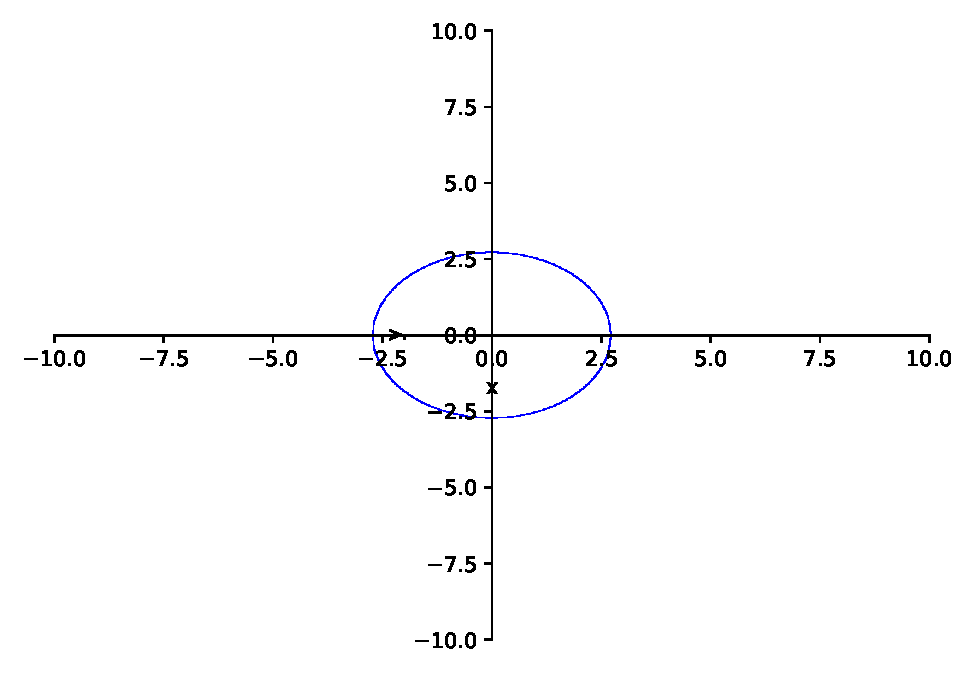
\includegraphics{ConformalMapping_files/figure-latex/unnamed-chunk-65-1.pdf}

When we hold \(c\) constant and vary \(\theta\), we obtain various curves constituting the family of logarithmic spirals of inclination \(\theta\). For all that follows, when we speak of logarithmic spirals of inclination \(\theta\), these are what we mean.

Let us show that, for any simply connected domain \(B\) that has boundary points, it is possible to map \(B\) onto the complex plane \(\mathbb{C}\) with a cut along an arc of a logarithmic spiral of inclination \(\theta\) in such a way that given points \(a\) and \(b\) of the domain \(B\) are mapped into \(0\) and \(\infty\), respectively. The expansion of the mapping function about \(z = b\) has the form:

\[ \frac{1}{z - b} +a_0+a_1{(z - b)} +\cdots\text{ or }  z+a_0+\frac{a_1}{z} +  + \cdots, \]

according as \(b\) is finite or infinite.

\begin{itemize}
\item
  If domain \(B\) has \textbf{a single boundary point},\\
  this is obvious, and then the arc of the logarithmic spiral referred to degenerates to a point.
\item
  If the boundary of the domain \(B\) is \textbf{a continuum},\\
  let us first map \(B\) conformally onto the domain \(\{z' : |z'| > 1\}\) in such a way that the point \(z = b\) is mapped into \(z' = \infty\).
\end{itemize}

Let \(z'\) be the mapping function \(cP(z)\) in a neighborhood of \(z = b\). The expansion can be expressed as:

\[
z' = cP(z) = \frac{1}{b} + \frac{1}{1} (z - b) + \frac{1}{1!} (z - b)^2 + \frac{1}{0!} (z - b)^3 + \ldots
\]

or

\[
z' = cP(z) = \frac{1}{b} + \frac{1}{1}z + \frac{1}{1!}z^2 + \frac{1}{0!}z^3 + \ldots
\]

depending on whether \(b\) is finite or infinite. This expansion is possible due to Riemann's theorem.

Suppose that the point \(z = a\) is mapped into a point \(z' = a'\). Now, we need to establish the possibility of mapping the domain \(\lvert z' \rvert > 1\) onto the complex plane with a cut along a logarithmic spiral of inclination \(\epsilon\). This possibility follows from solving the problem related to the minimum of the quantity:

\[
 \Re(e^{-2i\theta} \log (F'(a))
\]

in the class I. This problem was studied in Section 3 of Chapter IV (the first application of Theorem 1 with \(a = \frac{17}{2} - \epsilon\)). It was shown that this problem has a solution, and the extremal function (normalized by the condition \(F(a') = 0\)) provides the required mapping.

\begin{lemma}
\protect\hypertarget{lem:unnamed-chunk-66}{}\label{lem:unnamed-chunk-66}Of all functions
\[
\xi=F(z) := z + \frac{a}{z} + a_0 + \ldots
\]
that map the domain \(|z| > R\) univalently in such a way that a given finite point \(a\) and the point \(\infty\) are
mapped into the poi nts \(0\) and \(\infty\) respectively, the quantity \(\Re(e^{-2i\theta} \log (F'(a))\)
is minimized by the function \(F_0(z)\) that maps the disk \(|z| > R\) onto the \(\xi\)-plane with cut along an arc of a logarithmic spiral of inclination \(\theta\). Here \(\log F '(z)\) means the brooch that approaches \(0\) as \(z \to \infty\).
\end{lemma}

\begin{theorem}
\protect\hypertarget{thm:unnamed-chunk-67}{}\label{thm:unnamed-chunk-67}Every domain \(B\) in the \(z\)-plane can be mapped univalently onto a domain \(B'\) in the \(\omega\)-plane that includes the points 0 and \(\infty\), such that an arbitrary continuum of the complement of the domain \(B'\) with respect to the \(\omega\)-plane is an arc of a logarithmic spiral of given inclination \(\epsilon\). This mapping maps given points \(a\) and \(b\) of the domain \(B\) into 0 and \(\infty\), respectively, and the expansion of the mapping function about \(z = b\) has the form \((z - b)^{r_1} + a_0 + a_1 (z - b) + \ldots\) or \(z + a_0 + a_1 z^{-1} + \ldots\), according as \(b\) is finite or infinite.
\end{theorem}

  \bibliography{book.bib,packages.bib}

\end{document}
